\chapter{Validação de Novas Abstrações de Processos}
\label{cap:validacoes}

A maioria dos SOs oferecem a infraestrutura necessária para que os processos
existam. Eles precisam garantir (1) acesso aos recursos, (2) desempenho, (3)
segurança/isolamento e (4) funcionalidades adicionais (p.ex., mutexes).  Nesse
contexto, melhorias nos SOs devem trazer benefícios em alguma dessas frentes
buscando evitar o acréscimo de \emph{overhead}. Para testar as novas propostas de
abstrações, temos as opções de utilizar \emph{microbenchmarks} e aplicações
reais.  Aplicações reais são capazes de consumir CPU, realizar diversas
operações de leituras e escrita em disco, demandar muita leitura e escrita da
memória, gerar intenso tráfego de rede, causar muitas trocas de contexto (pela
paralelização), e podem comprometer os caches de memória e disco. Além disso,
algumas aplicações possuem necessidades específicas de segurança. Idealmente,
qualquer proposta de expandir a abstração de processos deve buscar formas de
validação que exercitem todas as características apresentadas.

Na prática, queremos algo que gere uma carga razoável de CPU, disco, rede e
paralelismo; além disso, que seja algo relativamente fácil de gerar carga e
medir o desempenho. Servidores web, atendem bem esses requisitos: são altamente
paralelos, geram bastante I/O e tráfego de rede, dependem de algum
processamento na CPU e há ferramentas para gerar carga e medir o desempenho. No
caso da segurança, faz sentido utilizar aplicações dedicadas, como
\emph{gnugpg} ou \emph{openssh}, e/ou uma biblioteca, como \emph{openssl}. Não
por acaso, quase todos os trabalhos que avaliamos usam alguma dessas
ferramentas para fazer suas validações.

O Capítulo \ref{cap:trabalhos-analisados} mostrou algumas pesquisas que buscam
estender a abstração de processos atual. Apesar dos vários trabalhos
demonstrarem algum tipo de benefício, muitos deles ignoram outros aspectos das
suas propostas. Por exemplo, uma abordagem que visa isolar dados para evitar
vazamento de informações faz testes que buscam por esses tipos de falhas, mas
deixam de avaliar se a alteração é viável em um contexto global com uma
demanda realista. Adicionalmente, alguns desses trabalhos baseiam-se
fortemente em \emph{microbenchmarks}, que podem evidenciar um resultado
desejado sem revelar um efeito colateral da alteração. Assim, surge a questão:
como avaliar de maneira mais completa e efetiva uma nova abstração? A resposta
advém indiretamente dos diversos trabalhos estudados. A ampla maioria das
propostas apresentadas no Capítulo~\ref{cap:trabalhos-analisados} alteraram uma
ou mais aplicações de uso cotidiano com o objetivo de demonstrar alguma
vantagem da alteração na abstração de processo sugerida. Contudo, sistematizar
quais aplicações e \emph{microbenchmarks} podem ser adotadas ainda é um questão
pouco discutida; por esse motivos levantamos e respondemos as seguintes
perguntas:

\begin{quote}
  \item \emph{QP3:.} ``Quais aplicações podem ser utilizadas para avaliar as novas abstrações adicionadas a um SO?''
  \item \emph{QP4:.} ``Qual conjunto de \emph{microbenchmarks} pode ser utilizado para auxiliar a entender os impactos de uma nova característica adicionada às abstrações de processos?''
\end{quote}


%Não vi a parte de \emph{microbenchmarks}, mas talvez você também possa argumentar
%algo como ``se é para validar com \emph{microbenchmarks}, precisamos ter um conjunto
%mínimo desses \emph{microbenchmarks} que todo mundo usa para minimizar as chances de
%efeitos colaterais indesejados escaparem''. Isso justificaria a existência da
%RQ4.
%}


Defendemos que uma das formas mais eficientes para validar uma nova extensão da
abstração de processos é por meio de aplicações já consagradas, amplamente adotadas por
diversos sistemas e que exercitam várias partes do SO. Por esses motivos,
buscamos extrair tais aplicações, dos trabalhos estudados no
Capítulo~\ref{cap:trabalhos-analisados}, que auxiliam na demonstração de que uma nova
proposta de abstração de processos é viável ou não. Buscamos três
características: estresse que a aplicação pode gerar, possíveis falhas de
segurança e áreas para otimização. Aplicações que consomem muitos recursos de
hardware são ideais para comprovar que uma nova extensão é escalável. Por outro
lado, várias propostas de novos mecanismos no processo prometem melhorias de
segurança e, por esse motivo, sistemas reais que já apresentaram alguma falha
de segurança são desejáveis para esse tipo de validação. Algumas pesquisas
propõem novos mecanismos dos quais alguns tipos de aplicações podem se
beneficiar, como por exemplo, novas formas de compartilhamento de memória e
otimizações. Nesses casos, é interessante utilizar alguma aplicação do tipo
adequado para a validação.
% TODO: Explicar o que é microbenchmark - validação Microbenchmarks têm por objetivo mensurar e fornecer meios para analisar uma única característica do objeto de estudo.
Outra perspectiva sobre a validação é representada pelos \emph{microbenchmarks}
que auxiliam no estudo dos impactos das alterações.  Esses testes são
vantajosos durante as etapas iniciais da implementação da nova abstração, uma
vez que são rápidos e podem ajudam durante o processo de desenvolvimento. Um
conjunto de \emph{microbenchmarks} pode ser usado para indicar que a nova
abstração traz vantagens, contudo, dado o seu alto nível de especialização, ele
não consegue revelar possíveis efeitos colaterais ou interferências com outras
funcionalidades.

A análise feita sobre as aplicações e \emph{microbenchmarks} foram originadas
dos diversos experimentos realizados pelos pesquisadores que mostramos no
Capítulo \ref{cap:trabalhos-analisados}. Além disso, durante esse trabalho,
foram conduzidos experimentos que auxiliaram na elaboração das ideias
apresentadas nesse capítulo. Esse capítulo pode ser dividido em duas partes:
aplicações e \emph{microbenchmarks}. Primeiramente apresentamos programas que
são favoráveis para serem adaptados de forma a utilizar as novas abstrações
de processos e, assim, servirem como mecanismo de validação para as propostas.
Tentamos ilustrar as características gerais das aplicações de forma a fornecer
ideias de possíveis adaptações (discutimos algumas delas
no Capítulo~\ref{cap:analise-sobre-abstracoes-de-processos}) e também prover
ferramentas para o leitor avaliar os trabalhos desse campo. Por fim,
apresentamos uma discussão sobre os potenciais \emph{microbenchmarks} que podem
ser utilizados para validar novas extensões nos processos.

% TODO: Eu acho que vale a pena fazer um parágrafo final dando uma visão geral
% sobre o que será discutido, mas especialmente falar que o Apache será mais
% detalhado devido ao estudo de caso do proxímo cap.

\section{Servidores Web}
\label{sec:web_server}

Muitos sistemas possuem máquinas dedicadas a uma aplicação específica com o
objetivo de entregar estabilidade, velocidade e estabilidade. Nesses casos, é
desejável que a CPU esteja ocupada a maior parte do tempo e use a memória de
forma eficiente para evitar desperdício de recursos. \boldAndIndex{Servidores
web} são aplicações que operam com um desempenho próximo
do ótimo utilizando boa parte dos recursos das máquinas para servir páginas
web. A principal responsabilidade do servidor web é entregar dados solicitados,
que podem vir de um arquivo ou ser gerados especificamente para cada
requisição. Uma requisição pode ser divida em três etapas: esperar por uma requisição
(\emph{request}) do usuário, processar a requisição e responder ao usuário.

\begin{figure}[!h]
  \centering
  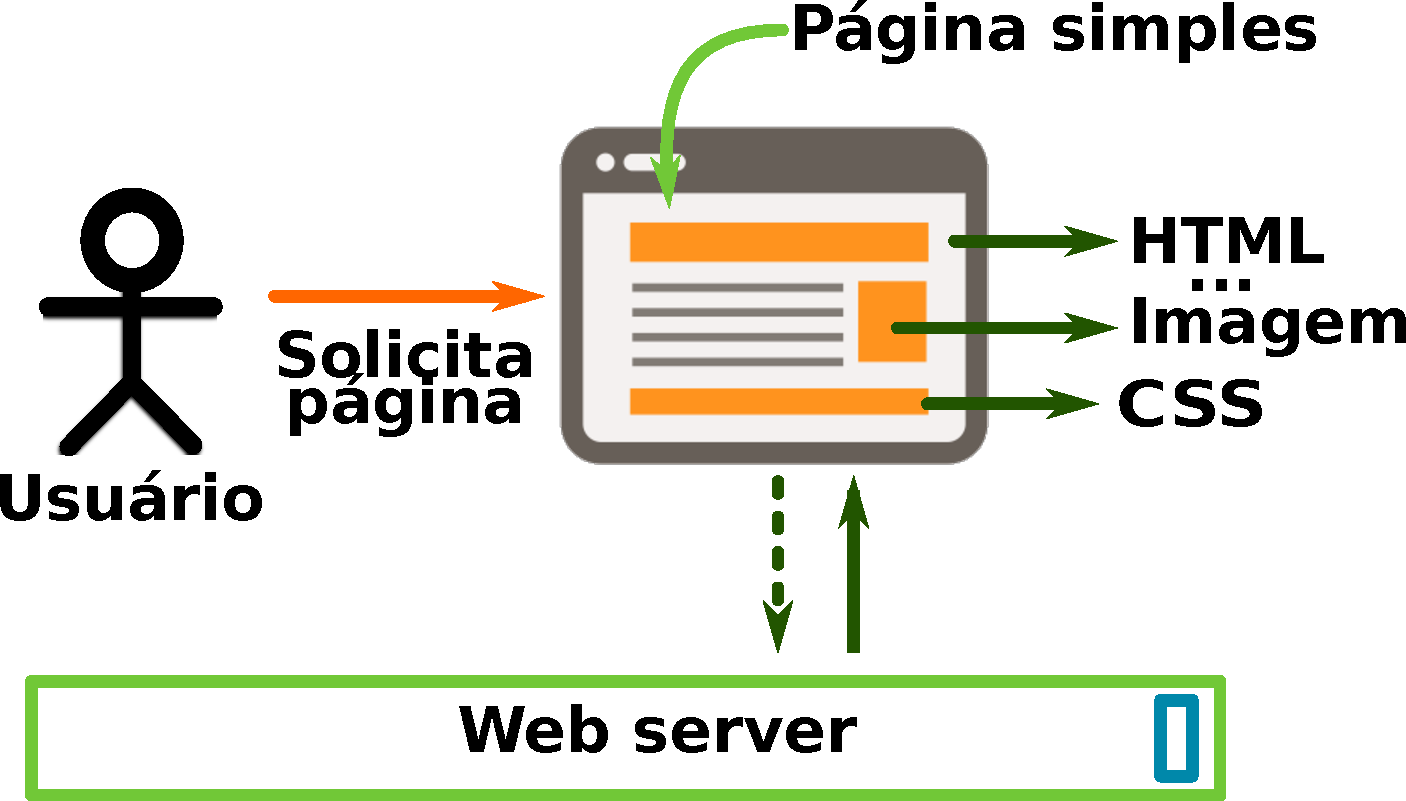
\includegraphics[width=.50\textwidth]{request_a_page}
  \caption[Do cliente para o servidor Web.]{Do cliente para o servidor Web. Note que o navegador solicita em paralelo os demais arquivos necessários para a construção da página.}
  \label{fig:client_to_web_server}
\end{figure}

A Figura \ref{fig:client_to_web_server} busca exemplificar uma situação simples
na qual o cliente solicita uma página web para um servidor. Inicialmente, o
cliente (digamos, um navegador web) comunica-se com o servidor através do
protocolo HTTP para fazer uma solicitação; por sua vez, o servidor responde
devolvendo os dados solicitado que contém todas as instruções básicas
necessárias para construir a página (HTML). O navegador abre o arquivo HTML
retornado, converte o conteúdo e verifica se precisa de mais informações para
construir a página solicitada; é comum que a página precise de outros arquivos
como CSS, imagens, javascript, etc. Se mais arquivos forem necessários, então o
navegador os solicita para o servidor de forma paralela ou serial. O exemplo
ilustra de forma simplificada como uma requisição acontece e como múltiplas
requisições podem ser geradas para construir uma simples tela. Um exemplo real
pode ser considerado da caracterização da carga gerada sobre o site da copa do
mundo de 1998, na qual foi gerado uma média de 10796
requisições/min~\citep{worldcup}.  Um servidor web tem que responder a milhares
de usuários e as estratégias utilizadas para lidar com tal volume são as mais
variadas.

Dado a enorme demanda que os servidores web precisam suportar, eles buscam
diversas técnicas que otimizem a utilização dos recursos. Uma das melhorias
disponíveis em alguns servidores web nasce da observação de que cada página a
ser apresentada para o cliente necessita realizar múltiplas conexões para obter
os vários arquivos que a compõem. Esse mecanismo de abrir e fechar
conexões constantemente impacta no desempenho uma vez que eleva a latência,
tempo gasto abrindo e fechando conexões. Uma possibilidade para minimizar esse
impacto é utilizar o mecanismo de \boldAndIndex{keep-alive}, que mantém uma
conexão aberta durante as atividades do usuário. Por exemplo, a Figura
\ref{fig:keep_alive} mostra um caso que não utiliza \emph{keep-alive} e outro
que utiliza. O primeiro caso ilustra uma situação padrão na qual uma requisição
é realizada e, por sua vez, são abertas e fechadas diversas outras conexões de
rede para obter cada um dos arquivos necessários para construir a página. O
segundo caso ilustra a técnica de \emph{keep-alive}, cujo o objetivo é reduzir
a latência e o uso de CPU no servidor mantendo a conexão aberta por um
intervalo de tempo.  Esse mecanismo pode melhorar a experiência do usuário ao
acessar o site em casos que um servidor esteja recebendo um elevado número de
requisições. Contudo, outro aspecto do \emph{keep-alive} é que ele pode elevar
o consumo de memória no servidor, gerando outro tipo de problema em um servidor
sobrecarregado. Esses dois mecanismos são importantes elementos a serem
considerados durante a realização de experimentos, uma vez que eles modificam o
comportamento geral do servidor em certas situações (retomaremos esse tópico no
Capítulo~\ref{cap:estudo-de-caso}).

\begin{figure}[!h]
  \centering
  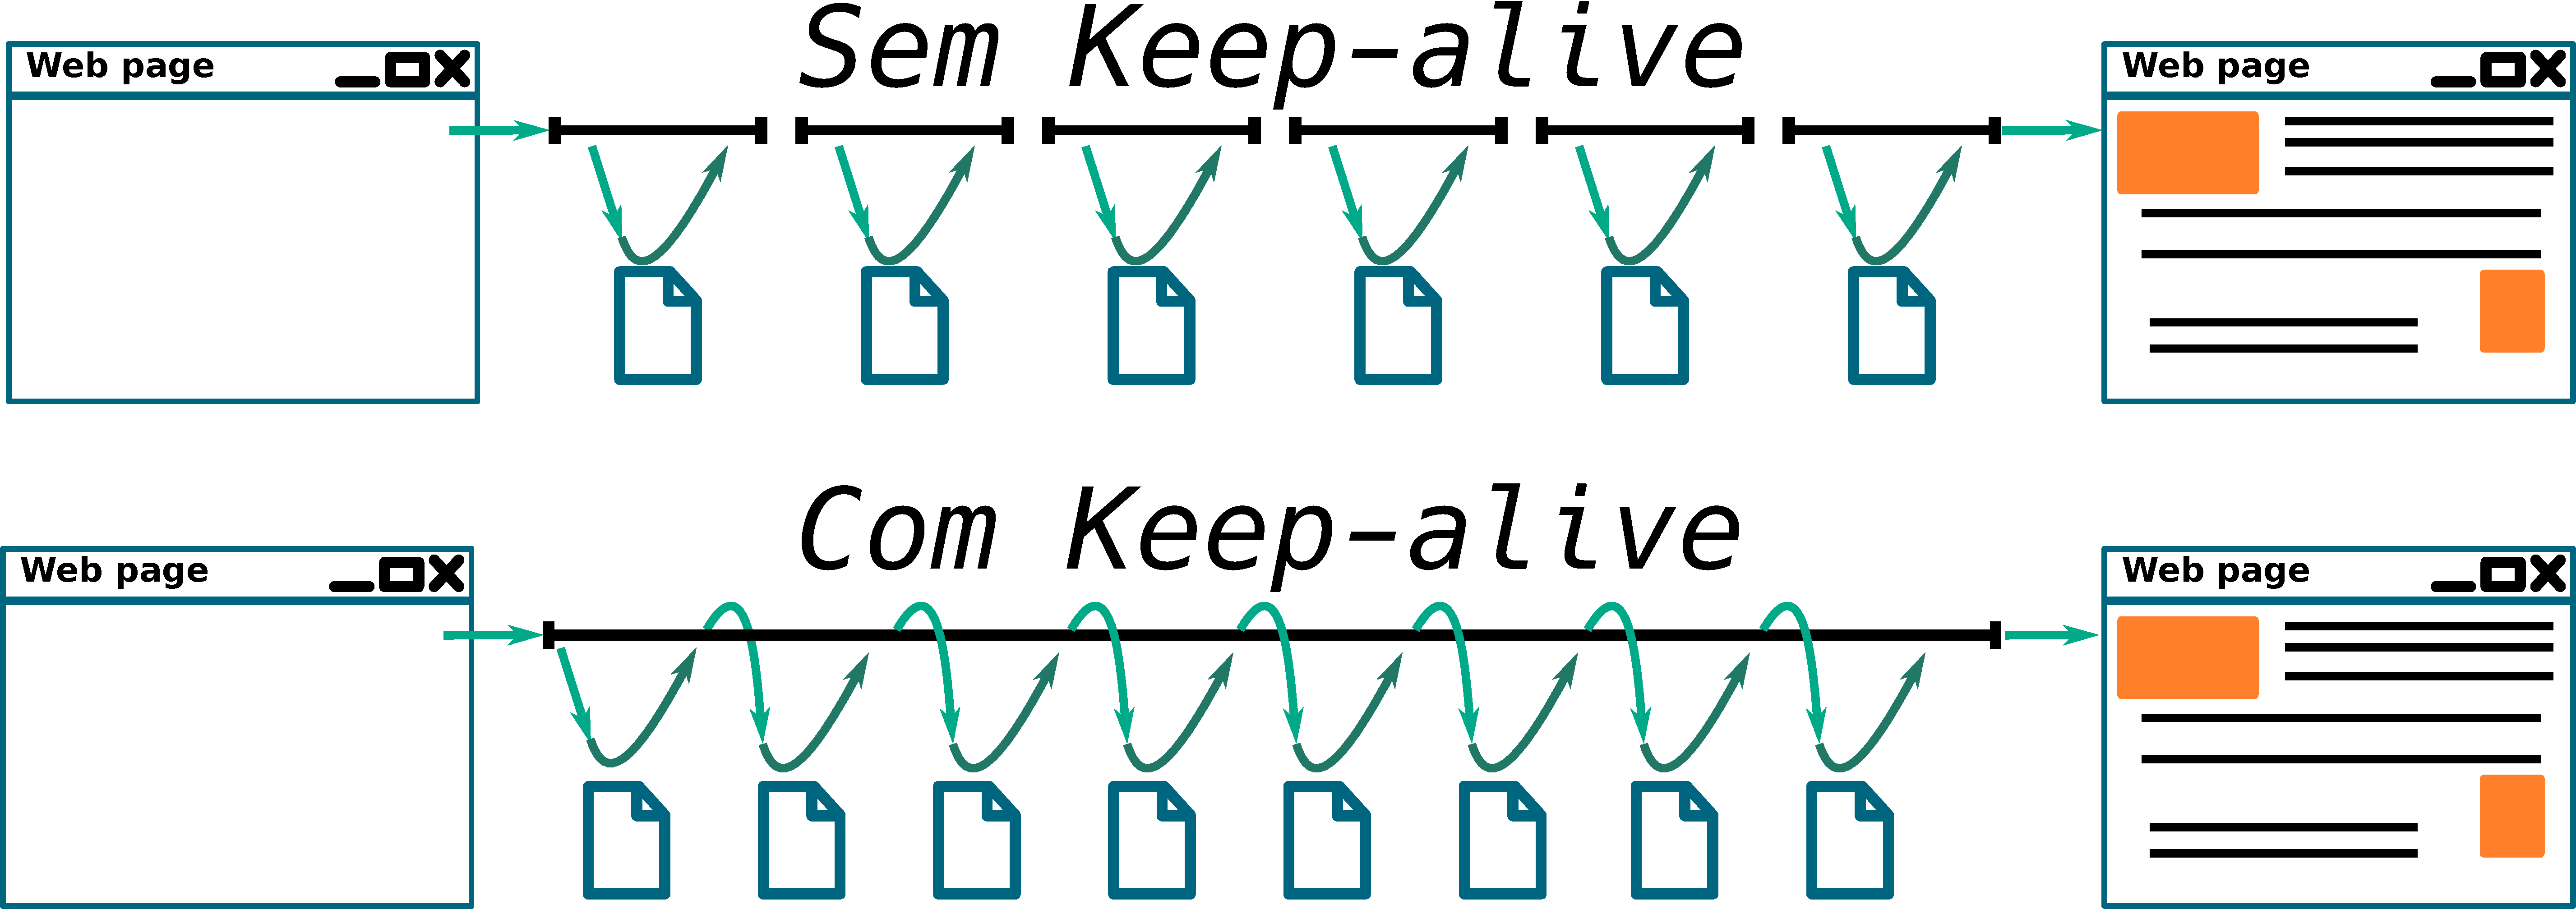
\includegraphics[width=\textwidth]{with_without_keep_alive}
  \caption{Exemplo de uma conexão feita sem \emph{keep-alive} e outra com \emph{keep-alive}}
  \label{fig:keep_alive}
\end{figure}

Existem muitos servidores web disponíveis no mercado, contudo, dois deles são
especialmente relevantes para o contexto deste trabalho:
Nginx\footnote{\url{https://www.nginx.com/}} e Apache
Httpd\footnote{\url{https://httpd.apache.org/}}.  O primeiro é conhecido pelo
seu bom desempenho para entregar arquivos estáticos, enquanto o segundo é conhecido
pela sua enorme estabilidade e comodidade. Ambos são amplamente usados,
extremamente configuráveis, confiáveis e suportam grandes cargas de
requisições. Trabalhos como \emph{Light-weight Contexts} e \emph{shreds}
fizeram uso desses servidores nos seus experimentos.

\subsection{Servidor Apache HTTPD}
\label{sec:architecture}

O servidor Apache HTTPD, também conhecido como \emph{HTTP Daemon (HTTPD)} é
licenciado com a licença Apache 2.0 e mantido pela fundação Apache.  O Apache
HTTPD\footnote{Usaremos HTTPD e Apache como sinônimos nesse texto.} foi
projetado para executar em vários SOs; essa restrição fez com que fosse
necessário adotar estratégias para fazer o HTTPD multiplataforma e mantendo um
bom desempenho. Uma característica importante do HTTPD é a sua forte separação
em módulos para manipular processos/\emph{threads} e outros elementos; o
conjunto de todos os módulos constituem a arquitetura do projeto. O Apache
utiliza a biblioteca \emph{Apache Portable Runtime (APR)}, cuja a intenção é
ser utilizada como uma interface portável para as tarefas comuns de programação
(p.ex.: alocação de memória, manipulação de tempo, etc). Por fim, o HTTPD
implementa um módulo especial chamado \emph{Multi-Processing Module (MPM)},
responsável por manter o processamento das requisições e a lógica de
manipulação de processos/\emph{threads}. O MPM é uma boa fonte de comparação entre
diferentes modelos de processos.

\begin{figure}[!h]
  \centering
  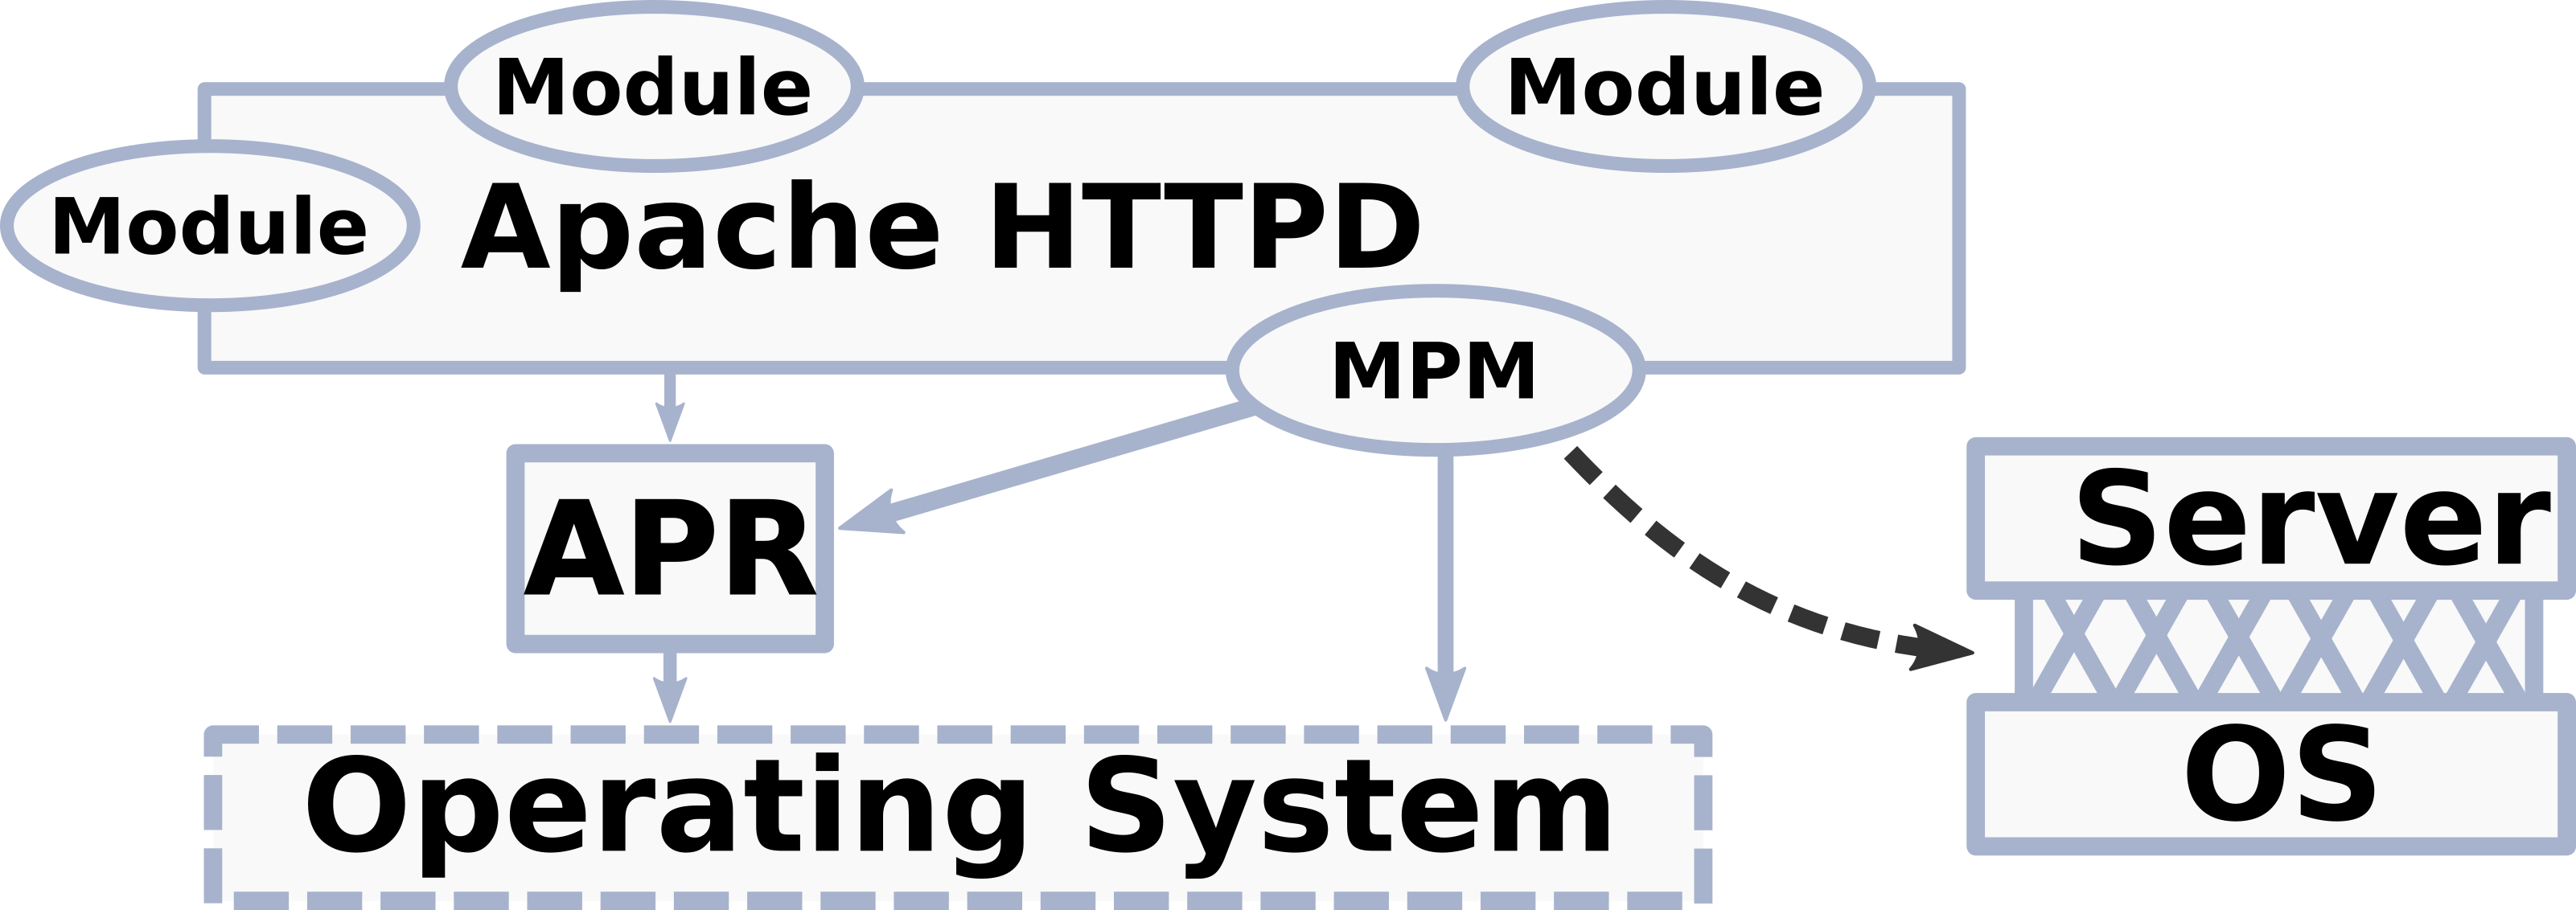
\includegraphics[width=.7\textwidth]{apache_arhitecture} 
	\caption[Arquitetura do servidor Apache HTTP]{Arquitetura do servidor Apache HTTP \citep{apache_module_book}}
  \label{fig:apache_architecture} 
\end{figure}

A Figura \ref{fig:apache_architecture} é uma visão de alto nível da arquitetura
do Apache. O topo da imagem representa os elementos do núcleo do Apache
responsáveis por juntar os demais componentes necessários para o seu
funcionamento. Ao redor do núcleo, existe um grande número de módulos anexados
que podem ser conectados ao projeto. Esses módulos facilitam o processo de
adicionar e remover elementos do núcleo, normalmente como bibliotecas
dinâmicas. Módulos na forma de bibliotecas dinamicamente ligadas fornecem
flexibilidade, um bom desempenho e portabilidade entre diferentes SOs (p.ex.,
Window e Linux podem ter diferentes implementações para o mesmo módulo). A
Figura \ref{fig:apache_architecture} também ilustra o MPM como um componente
diretamente conectado ao SO, porque o MPM manipula os elementos de
paralelização e cada SO precisa implementar essa parte de acordo com as suas
próprias particularidades. A última parte da imagem mostra a biblioteca APR,
que se posiciona entre o núcleo do HTTPD e o SO.

\begin{figure}[!h]
  \centering
  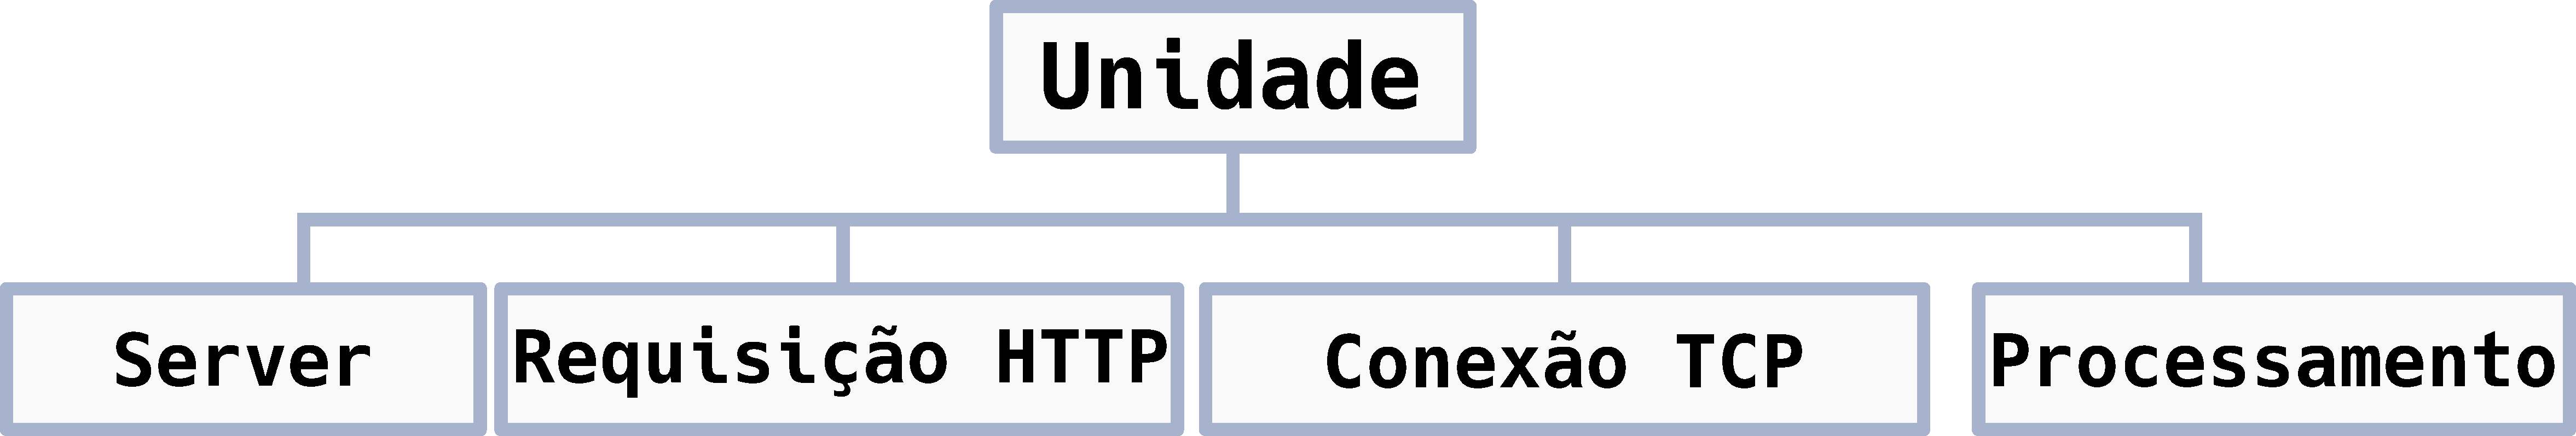
\includegraphics[width=.7\textwidth]{units} 
  \caption{Componentes do Servidor Apache HTTP}
  \label{fig:units} 
\end{figure}

Alguns módulos são essenciais para o funcionamento do HTTPD, uma vez que eles
representam os elementos básicos das estruturas de dados que são usadas por
todo o código. A Figura \ref{fig:units} mostra alguns componentes fundamentais
usadas pelo HTTPD. O módulo \emph{server} é responsável por criar uma estrutura de
dados para a requisição toda vez que o HTTPD aceita uma nova conexão. O módulo
HTTP é encarregado de preencher uma estrutura de dados de requisição e o
módulo de conexão TCP constrói a estrutura de dados que mantém as informações
da conexão. Normalmente, não é preciso se preocupar com módulos relacionados
aos detalhes do HTTP, uma vez que o Apache ajusta todos os elementos necessários
e também entrega uma estrutura de dados pronta para ser utilizada.

\begin{figure}[!h]
  \centering
  \includegraphics[width=.9\textwidth]{request_phases} 
	\caption[Gerador de Conteúdo]{Gerador de Conteúdo \citep{apache_module_book}}
  \label{fig:content_generator} 
\end{figure}

Outros dois aspectos da arquitetura do Apache são o \textbf{Content Generator}
(Gerador de Conteúdo) e as fases de processamento das requisições. O
\emph{Content Generator} pode ser visto como o núcleo do Apache, uma vez que
ele é responsável pelas operações de escutar por requisições e devolver
respostas; existe exatamente um gerador de conteúdo por requisição. No Apache,
um módulo pode registrar um \emph{content generator} de forma simples (basta
ajustar o \texttt{httpd.conf}) e, se nenhum estiver disponível, ele utiliza
o gerador padrão que simplesmente mapeia um arquivo para uma requisição
\citep{apache_module_book}. O \emph{content generator} pode processar toda a
requisição sozinho, contudo o Apache divide a \emph{request} em várias fases
como pode ser visto na Figura \ref{fig:content_generator}. Alterações nessas
fases podem ser extremamente proveitosas para testar novas abstrações de
processos.

\subsubsection{MPM}
\label{sec:prefork}

O módulo \emph{Multi-Processing (MPM)} é um elemento especial dentro do Apache.
Como a Seção \ref{sec:architecture} introduziu, o MPM funciona como uma
interface entre o HTTPD e o SO. O MPM tem três características principais para
qualquer instância do Apache: deve ser único, é obrigatório e tem uma
implementação específica para o SO alvo. O HTTPD fornece pelo menos um módulo
MPM por SO; por exemplo, Windows utiliza \texttt{mpm\_winnt} e Linux tem três
opções diferentes. Cada uma delas pode ser classificada como baseada em
processos ou em \emph{threads}. São elas: \emph{Prefork}, \emph{Worker} e
\emph{Event}. Esses módulos constituem bons pontos para comparar \emph{threads}
e processos usando as novas abstrações, uma vez que apenas um ponto isolado do
Apache é alterado; isso faz com que o comportamento padrão do HTTPD seja
conservado e assim a comparação entre diferentes abordagens ocorra de forma
mais justa. Em outras palavras, alterar o módulo de multi-processamento do
Apache conserva o ambiente de teste e fornece comparações mais precisas.

\begin{description}

	\item[Prefork:]

foi a primeira estratégia adotada pelo HTTPD e é totalmente
baseado em processos. A Figura \ref{fig:prefork} ilustra os três passos
realizados pelo \emph{Prefork}. O Apache inicia com um processo responsável
por gerir os filhos que serão encarregados de manipular uma requisição por vez.
Em seguida, ao receber uma requisição, o processo de controle identifica um
processo filho que esteja ocioso e repassa a requisição para ele, que
se encarrega da tarefa de tratar a solicitação. Caso não exista nenhum
processo filho disponível para manipular a requisição, o processo de
controle cria novos processos filhos. Repare que o processo de controle
comporta-se como um balanceador de carga.

\begin{figure}[!h]
  \centering
  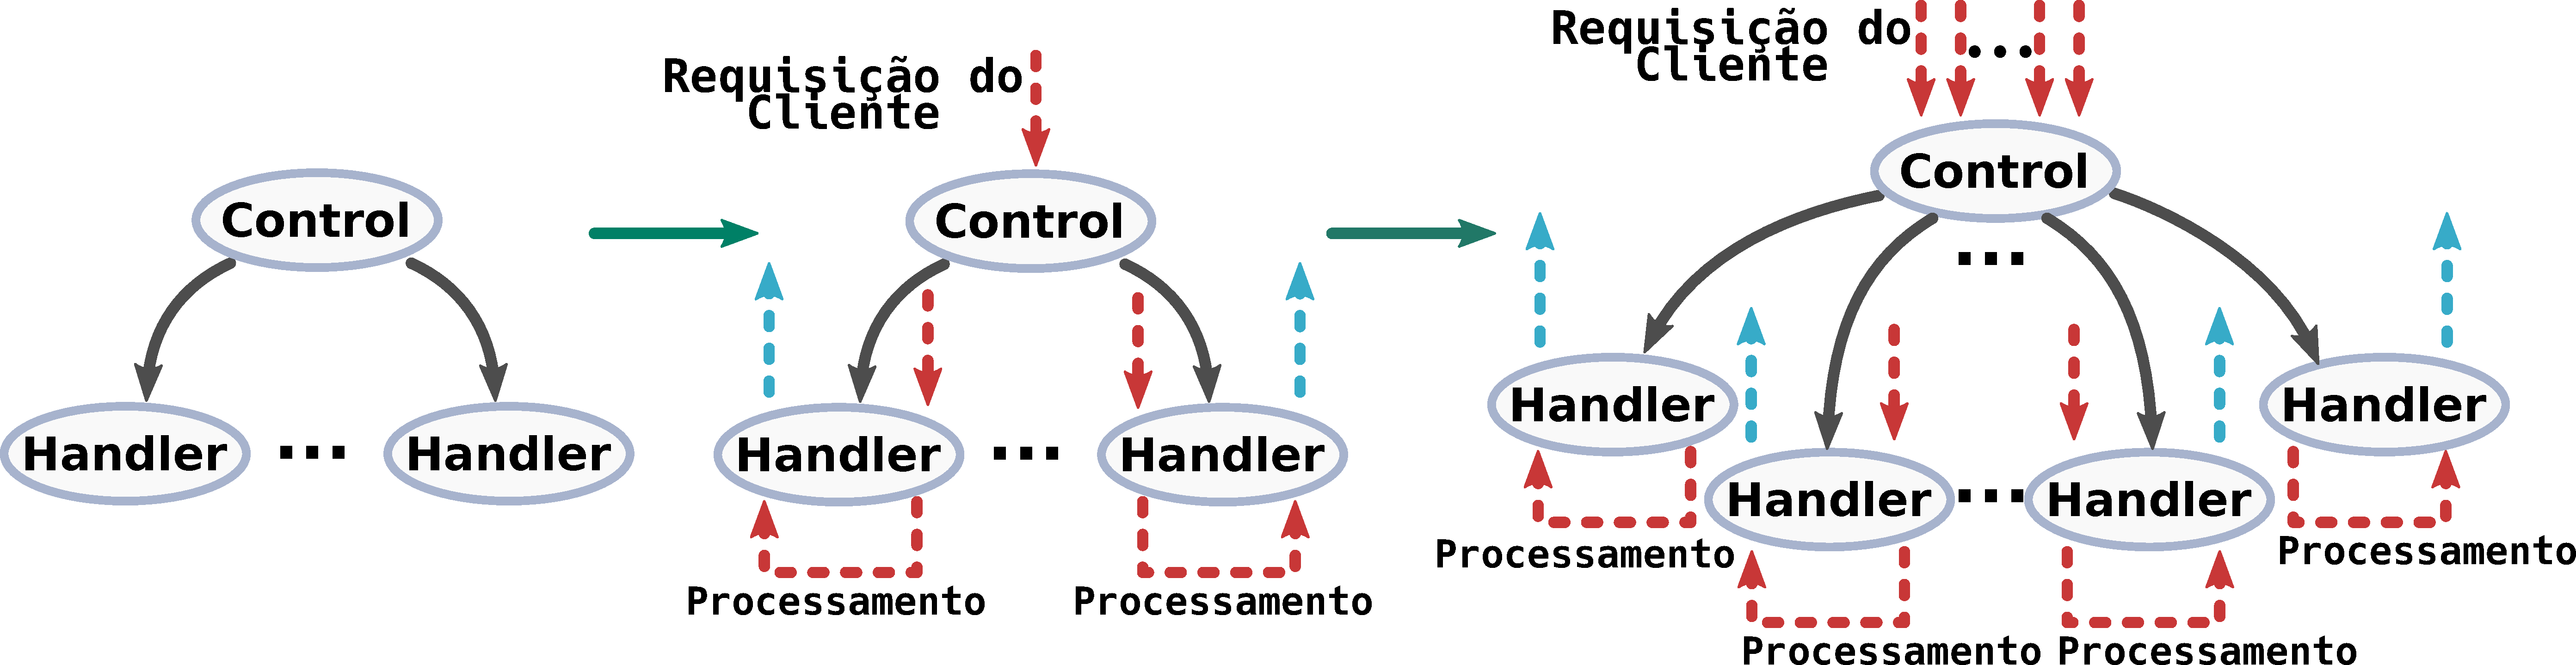
\includegraphics[width=\textwidth]{prefork} 
  \caption{Prefork}
  \label{fig:prefork} 
\end{figure}

\emph{Prefork} é uma boa opção para servidores web que não são compatíveis
com \emph{threads} (p.ex., pela utilização de aplicações legadas escritas em PHP) e é a melhor opção de MPM
para isolar requisições recebidadas pelo Apache. Contudo, \emph{Prefork} consome muita
memória e CPU, o que não é desejável em um servidor sob forte demanda.

  \item [Worker]: é uma solução híbrida, uma vez que seu
\emph{design} é baseado em processos e \emph{threads}. Esse módulo tem um
processo de controle que também é responsável por criar processos filhos e
controlar o balanceamento da carga entre eles.  Ao contrário de \emph{Prefork},
\emph{Worker} não cria instâncias de processos filhos para manipular
requisições feitas pelos clientes: ao invés disso, cada filho possui várias
\emph{threads} para realizar o tratamento das requisições. Comumente, o HTTPD
tem que manipular uma grande carga de requisições e, nesses casos, o processo
de controle age criando novos filhos (cada um com um conjunto de
\emph{threads}) para suportar a carga.  Repare que \emph{Worker} utiliza
\emph{threads} para manipular as requisições, fazendo com que o total de
processos filhos criado seja relativamente pequeno (comparado com o
\emph{Prefork}) e, consequentemente, o consumo de memória seja reduzido. O
HTTPD tem um arquivo de configuração que permite um controle fino de todos os
parâmetros relacionados ao número máximo de processos filhos, o total de
\emph{threads} por filho, dentre outros.

\begin{figure}[!h]
  \centering
  \includegraphics[width=\textwidth]{worker} 
  \caption{Worker}
  \label{fig:worker} 
\end{figure}

A Figura \ref{fig:worker} é um exemplo de como o \emph{Worker} funciona.
Quando o Apache inicia, ele tem um processo de controle e alguns processos
filhos que mantêm um grupo de \emph{threads} paradas. A segunda parte da figura
representa o caso em que o HTTPD recebe um grande número de requisições e o
processo de controle cria mais filhos para suportar a carga. O \emph{Worker}
consome menos memória que o \emph{Prefork} e, consequentemente, é melhor em
casos nos quais o servidor está sobrecarregado.  A mistura de processo e \emph{thread}
adiciona estabilidade para todo o sistema.

  \item [Event:] O módulo \emph{Event} é baseado em \emph{threads} e é o padrão
na última versão do Apache. A Figura \ref{fig:event} ilustra o comportamento
básico de \emph{Event}. A forma na qual \emph{Event} opera é similar à do
\emph{Worker}, contudo esse mecanismo diferencia-se por dois elementos extras:
mecanismo de manipulação do \emph{keep-alive} e separação da responsabilidade
de transmitir os dados para o cliente. O processo extra, incumbido de enviar as
informações para o cliente, comunica-se com as diversas \emph{threads} que
manipulam as requisições e tomam para si a responsabilidade de enviar os dados
processados.

\begin{figure}[!h]
  \centering
  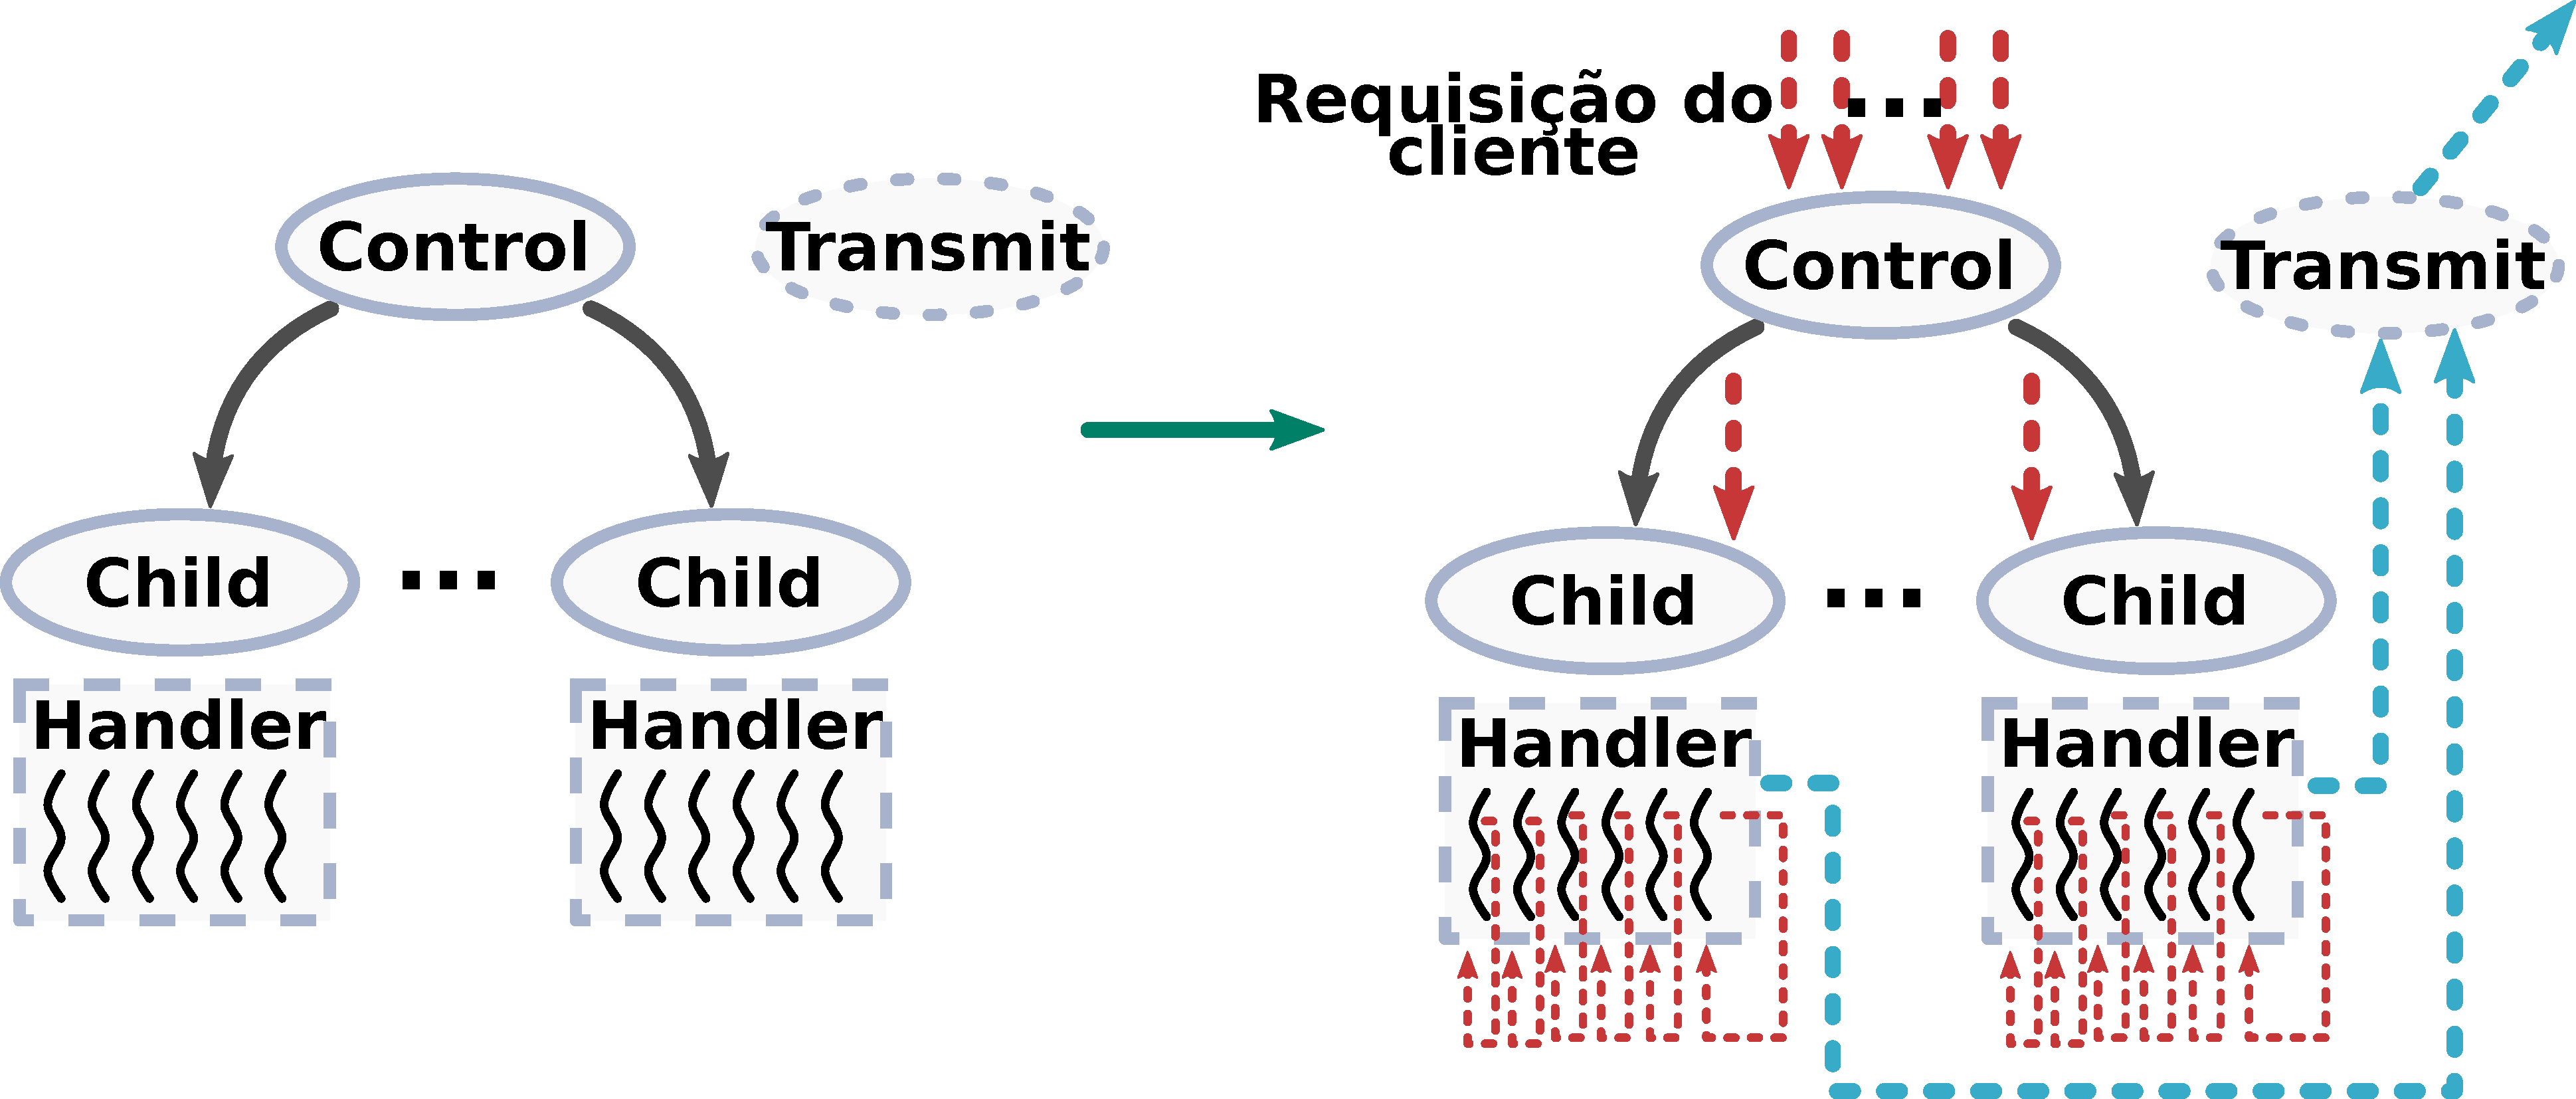
\includegraphics[width=.7\textwidth]{event} 
  \caption{Event}
  \label{fig:event} 
\end{figure}

\end{description}

\subsection{Nginx}

Assim como o Apache HTTPD, Nginx é um servidor web, contudo ele diferencia-se
de muitas formas dos servidores web tradicionais. A sua principal
característica é o seu excelente desempenho para atender requisições,
principalmente aquelas relacionadas a arquivos estáticos. Além disso, o Nginx
é comumente usado como um \emph{reverse-proxy}; ele recebe uma requisição do
usuário, por sua vez ele repassa a requisição para uma aplicação específica
responsável por realizar o processamento (p.ex. Puma, PHP-FPM, etc). Quando o
dado é processado pela aplicação, ela devolve o resultado para o Nginx, que
repassa os dados para o usuário \citep{soni}. A Figura \ref{fig:nginx_basico}
ilustra o funcionamento geral do Nginx; note que, neste exemplo, a requisição
do usuário chega ao servidor criptografada por meio do protocolo SSL
(vide Seção \ref{sec:openssl}). Em seguida, o Nginx
trata a solicitação transformando-a em HTTP; por fim, o processo termina
repassando-a para algum serviço.

\begin{figure}[!h]
  \centering
  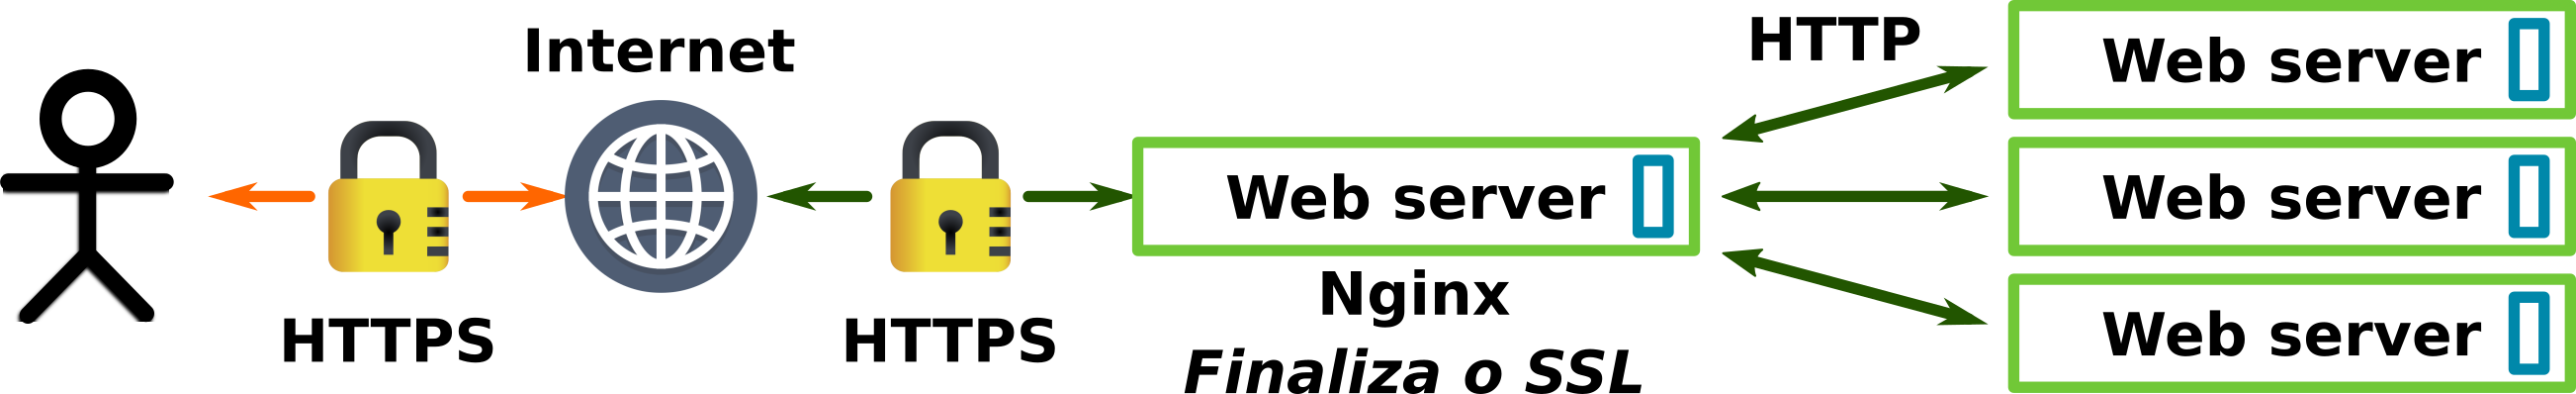
\includegraphics[width=\textwidth]{nginx_load_balancer_ex} 
  \caption[Nginx comportando-se como reverse-proxy]{Nginx comportando-se como reverse-proxy \citep{soni}}
  \label{fig:nginx_basico} 
\end{figure}

A grande maioria dos servidores web, inclusive o Apache, busca tirar o máximo
de proveito dos recursos de hardware utilizando um elevado número de
\emph{threads} e processos. Essa abordagem é relativamente simples de ser
implementada e traz bons resultados, contudo também tem alguns problemas.
Dentre as desvantagens, o modelo baseado em \emph{threads}/processos gera uma
grande quantidade de operações que bloqueiam e, consequentemente, geram trocas
de contexto. Além disso, a abordagem baseada em \emph{threads}/processos
consome uma elevada quantidade de recursos (p.ex. memória, descritores de
arquivos e CPU), degradando o desempenho da aplicação em situações de elevada
demanda.

O Nginx utiliza uma outra abordagem de servidor web, baseada na ideia de eventos;
esse mecanismo, é uma técnica baseada em requisições de I/O assíncronas. Por
uma questão histórica o Apache não faz uso desse método pois as operações de
I/O assíncronas não funcionavam bem nas suas primeiras versões no Linux. A
estratégia de eventos parte do princípio de que deve-se evitar ao máximo a
troca de contexto e, assim, tirar o máximo de proveito da CPU com processamento
útil.  Por esse motivo, Nginx cria apenas três tipos de processos
\citep{nginx_architecture}:

\begin{itemize}
  \item Processo mestre, que faz operações privilegiadas como ler arquivos de configuração e acessar portas;
  \item Processo de cache de disco, que carrega dados do disco fazendo cache na memória;
  \item Processo gestor de cache, que gerencia o cache e que realiza verificações sobre ele periodicamente;
  \item Processos \emph{Worker}, que fazem o trabalho de manipular conexões, ler e escrever em disco e comunicar-se com os clientes.
\end{itemize}

Nginx recomenda um \emph{Worker} por núcleo da CPU, o que permite tirar
grande proveito dos eventos.

Na prática, o sistema de eventos é eficiente pois gera poucos bloqueios
(comparado com o modelo que utiliza \emph{threads}/processos), uma vez que não espera
a aplicação terminar o que está fazendo para iniciar outra atividade. Por
exemplo, se o \emph{worker} estiver atendendo uma requisição e, em um
determinado momento, precisar recuperar uma informação do disco, ele não
bloqueia, mas simplesmente vai fazer outra tarefa e salva o evento referente à
busca no disco para retornar a ele depois (mais precisamente, quando surgir um
evento). O sistema de eventos faz com que um único \emph{worker} execute
múltiplas tarefas de forma sequencial sem bloqueio e, consequentemente, com
poucas trocas de contexto.

\section{Ferramentas de Comunicação Criptografada}
\label{sec:com_enc}

Como mostrado no Capítulo \ref{cap:trabalhos-analisados}, algumas das novas
propostas de abstrações de processos levam melhorias de segurança para o espaço
de usuário. Nesse sentido, aplicações que envolvem mecanismos de criptografia
ou que têm algum requisito especial de segurança representam bons casos de uso
para validar novas abstrações. Esse tipo de software costuma ser desenvolvido
por uma comunidade de especialistas na área de segurança, o que significa que
levar melhorias a esse tipo de ferramenta não é uma tarefa trivial. Por uma
questão de simplicidade e abrangência selecionamos dos diversos trabalhos
discutidos no Capítulo~\ref{cap:trabalhos-analisados}, duas ferramentas
amplamente utilizadas: OpenSSH e OpenSSL.

\subsection{OpenSSL}
\label{sec:openssl}

Antes de discutir o pacote OpenSSL, é importante apresentar de forma geral o
protocolo \boldAndIndex{Secure Sockets Layers (SSL)}. O principal objetivo de
SSL é fornecer um conjunto de protocolos criptográficos que permita a
comunicação segura em rede. É uma ferramenta de uso cotidiano, e diversas
aplicações críticas à missão dependendo dele, o que o torna um constante alvo
de ataques (existem mais de 200 CVEs reportadas para essa
ferramenta\footnote{\url{https://cve.mitre.org/cgi-bin/cvekey.cgi?keyword=OpenSSL}}).

O SSL utiliza um mecanismo chamado \boldAndIndex{handshake}, que
nada mais é do que um processo de negociação entre o cliente e o servidor de uma conexão de rede, de
forma a criar uma conexão segura entre ambos. A Figura
\ref{fig:openssl_handshake} descreve de forma geral os passos da negociação. O
processo de \emph{handshake} começa com o cliente mandando uma mensagem do
tipo ``Oi, sou o cliente'' para o servidor; nessa mensagem, o cliente informa a
versão do SSL que está usando, os algoritmos de criptografia e os métodos de
compressão que ele sabe manipular. O servidor, por sua vez, responde com ``Oi, sou o
servidor'', dizendo qual algoritmo usar (selecionado da lista que o cliente
mandou), um ID da seção, um certificado digital e a sua chave pública. Com o
certificado, o cliente consulta uma Autoridade Certificadora (\emph{Certificate Authority -- CA})
que valida se o servidor é valido ou não,
estabelecendo a confiança sobre o servidor. Depois que o cliente recebe a
validação da CA, ele começa a etapa de troca de chaves, na qual o cliente envia
uma chave secreta compartilhável. O cliente criptografa essa chave com a chave
pública fornecida pelo servidor antes do envio e termina enviando uma mensagem de
fim. O servidor decriptografa a mensagem do cliente e utiliza a chave enviada
para criptografar uma mensagem de fim para ser enviada para o cliente. Quando
o \emph{handshake} termina, o servidor e o cliente podem enviar mensagens que
são simetricamente criptografadas com a chave compartilhada \citep{openssl}.

\begin{figure}[!h]
  \centering
  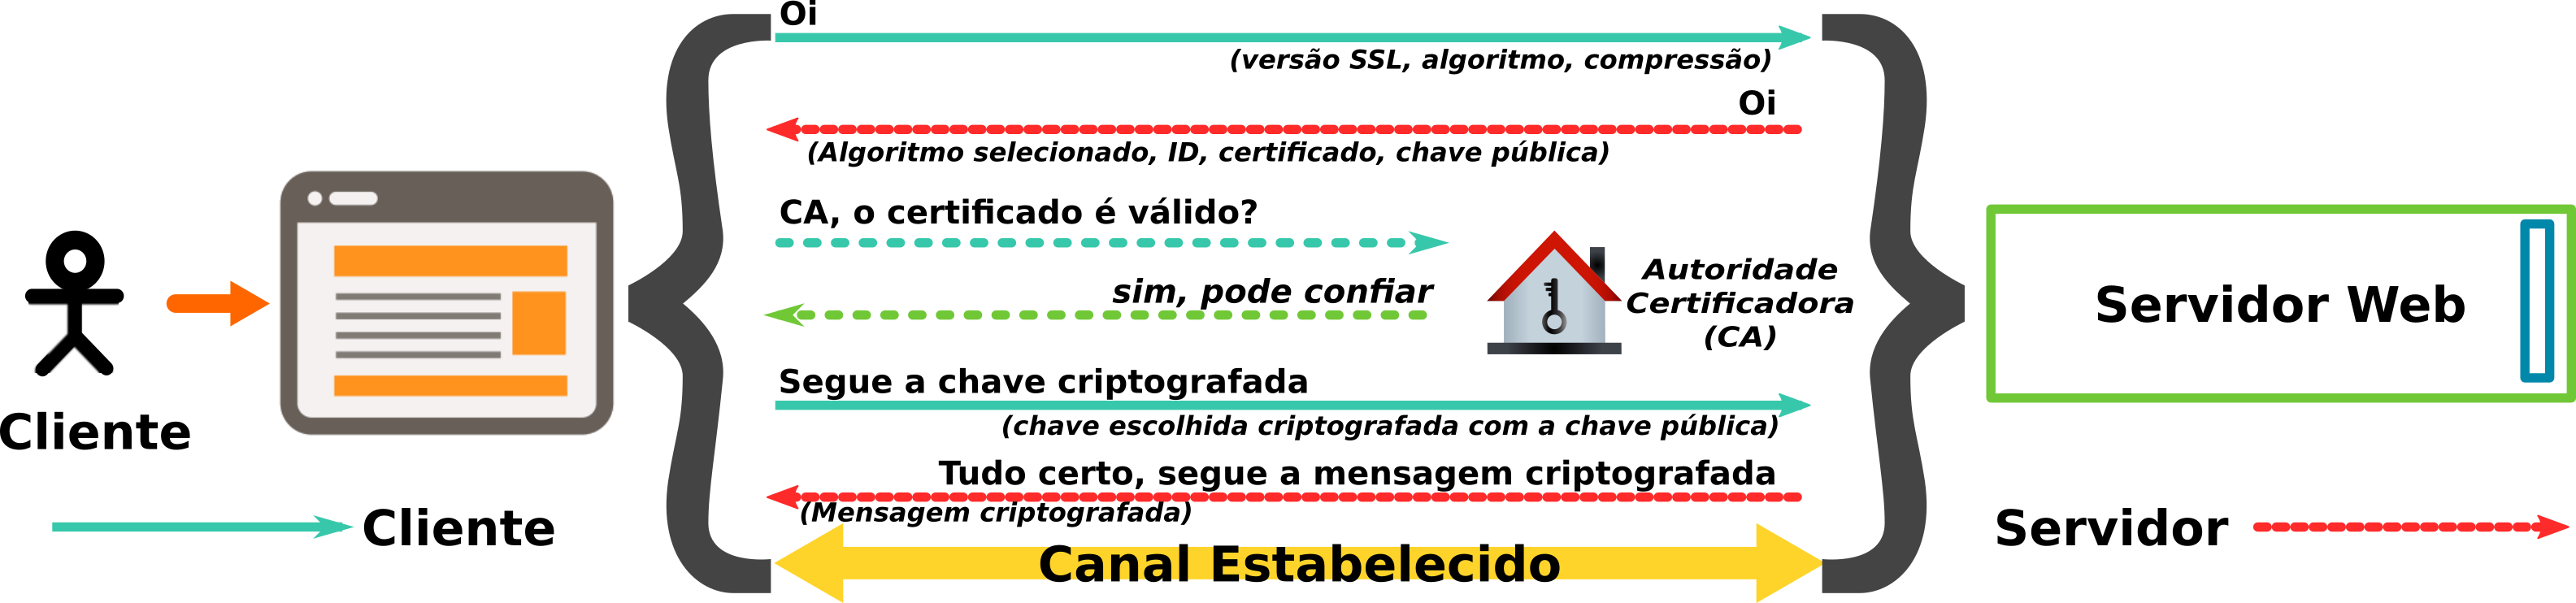
\includegraphics[width=\textwidth]{ssl_handshake}
  \caption{Do cliente para o servidor Web}
  \label{fig:openssl_handshake}
\end{figure}

O OpenSSL é uma implementação livre do protocolo SSL que
inclui várias funções criptográficas e utilitárias. A Figura
\ref{fig:openssl_arch} mostra uma visão geral da arquitetura do OpenSSL. O
\emph{EVP crypto API} são funções de alto nível que fornecem recursos para
derivação de chaves, \emph{hash} seguro, código de autenticação de mensagens,
criptografia/decriptografia de algoritmos simétricos/assimétricos, dentre outros. A
arquitetura também fornece uma pilha de manipulação de erros e uma interface
abstrata para lidar com I/O.

\begin{figure}[!h]
  \centering
  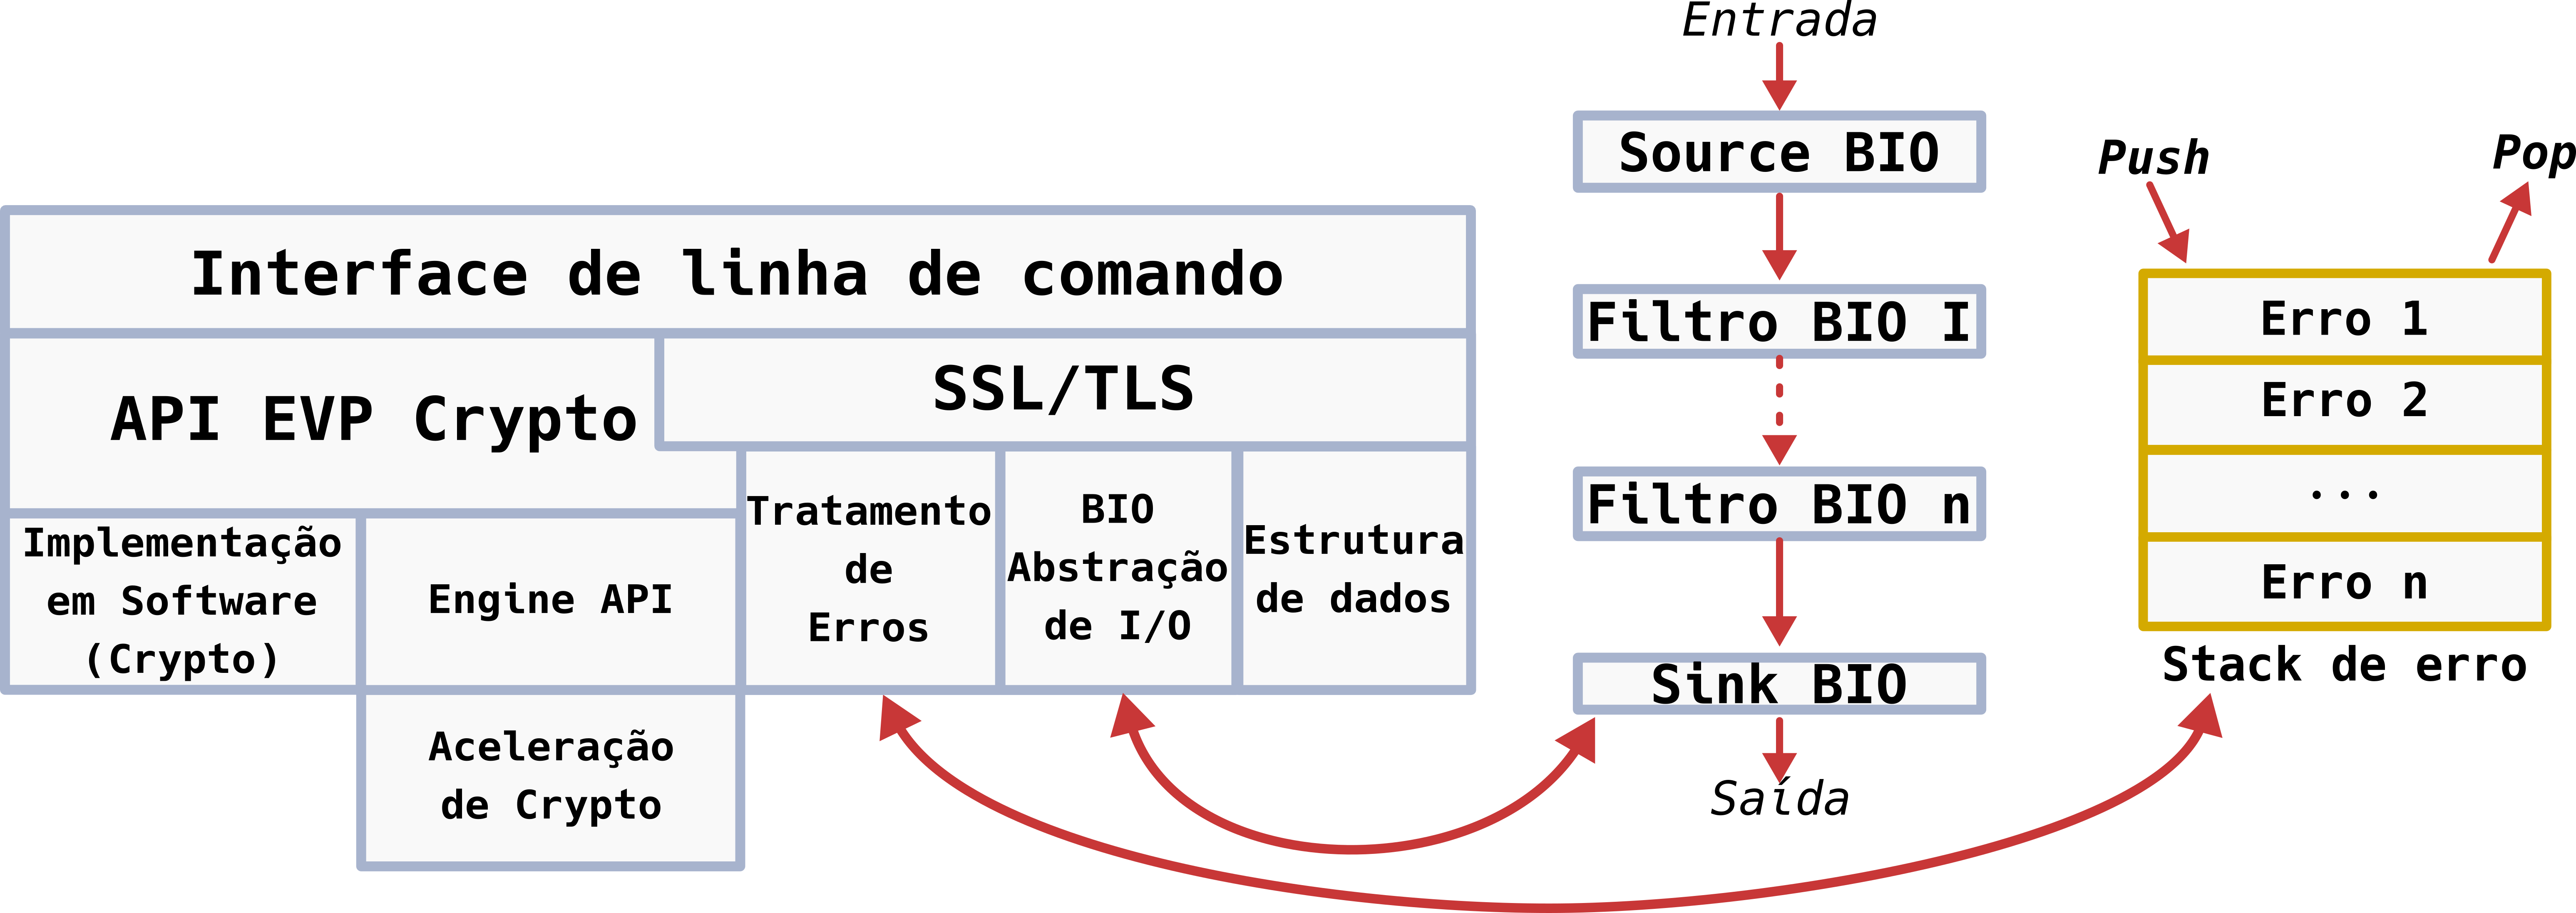
\includegraphics[width=\textwidth]{openssl_arch}
  \caption[Arquitetura do OpenSSL]{Arquitetura do OpenSSL \citep{crypto_openssl}}
  \label{fig:openssl_arch}
\end{figure}

Dado a sua versatilidade e constante aprimoramento, o OpenSSL tornou-se uma das
ferramentas mais utilizadas por diversos projetos consagrados. Dentre eles
destacam-se:

\begin{description}
  \item [Apache-SSL/mod\_ssl:] módulo do Apache que fornece suporte para utilizar protocolos de criptografia;
  \item [Net::SSLeay:] módulo \emph{Perl} que funciona como uma interface para as operações fornecidas pelo OpenSSL sendo amplamente utilizado por diversas aplicações escritas em \emph{Perl};
  \item [cURL:] software que fornece uma biblioteca e ferramentas de linha de comando para transferir dados usando diversos protocolos (p.ex., FTP, HTTP, HTTPS, GOPHER e DICT); 
  \item [Samba:] popular sistema de compartilhamento de arquivos integrado com vários clientes;
  \item [OpenSSH:] conjunto de utilitários que fornece um canal seguro de comunicação em rede (discutiremos sobre essa ferramenta na próxima seção).
\end{description}

As aplicações citadas acima representam apenas algumas das ferramentas que
utilizam o OpenSSL, note que alterações nessa biblioteca impactam diretamente
em uma ampla variedade de ferramentas. Dado a sua vasta utilização, várias
vulnerabilidades foram encontradas e catalogadas na forma de \boldAndIndex{Vulnerabilidades e
Exposições Comuns (\emph{Common Vulnerabilities and Exposures} - CVE)}. A CVE é
um sistema que fornece de forma pública e metodológica, informações sobre uma
vulnerabilidade conhecidas. Dentre as CVEs registradas do OpenSSL destacamos
apenas duas com o objetivo de ilustrar como abrações de processos podem
demonstrar melhorias na prática, segue:

\begin{description}
  \item [Heartbleed:] Das versões 1.0.1 até 1.0.1f do OpenSSL é possível
encontrar uma falha de segurança chamada de \textbf{Sagramento do Coração};
essa falha nasce de um erro de implementação, em uma extensão chamada de
\emph{heartbeat} (batida do coração). O \emph{heartbeat} é um mecanismo que
permite ao cliente manter a conexão segura por mais tempo, para isso o cliente
solicita um byte de informação toda vez que tenta manter a conexão (``batimento
do coração''). Contudo, o OpenSSL cegamente acreditava no valor solicitado sem
realizar qualquer tipo de validação; isso permitia que alguém solicitasse mais
dados da memória do que o permitido (``sangramento do coração''). Essa falha
permite que um agressor consiga roubar ou vazar informações como nomes e
senhas de usuários; em casos extremos, pode ser possível recuperar a chave
privada usada pelo OpenSSL\footnote{\url{https://cve.mitre.org/cgi-bin/cvename.cgi?name=CVE-2014-0160}}.

  \item [CCS Injection Vulnerability:] As versões 0.9.8za, 1.0.0m e 1.0.1h do
OpenSSL são comprometidas com essa falha. Essa vulnerabilidade pode ser
explorada por um atacante que fique entre o cliente e o servidor.  Basicamente,
o agressor captura as requisições feitas durante o \emph{handshake}
(Figura~\ref{fig:openssl_handshake}) e manipula a chave que será usada para
criptografar o tráfego. Essa falha ocorre devido a fraquezas no método de gerar
chaves
\footnote{\url{https://cve.mitre.org/cgi-bin/cvename.cgi?name=CVE-2014-0224}}.

\end{description}

Propostas de extensão da abstração de processos que pretendem trazer melhorias de
segurança, podem utilizar versões comprometidas do OpenSSL e tentar mostrar que
a nova abstração resolve um problema real. O pesquisador pode consultar a longa
lista de CVEs, selecionar um dos problemas, replicar e em seguida resolver a
falha utilizando a sua proposta. Dado a ampla utilização do OpenSSL, fica claro
o impacto de propostas que tragam melhorias de segurança para tal ferramenta.

\subsection{OpenSSH}

Uma das tarefas mais comuns do dia-a-dia de muitos desenvolvedores e
administradores de sistemas, consiste em acessar servidores em diversos locais
do mundo e configurar uma determinada aplicação. Na prática, boa parte dos
profissionais de TI faz uso de conexões seguras na Internet por meio do
protocolo \emph{Secure Shell (SSH)}. Existem diversas implementações desse
protocolo, mas para este trabalho discutiremos o OpenSSH.

A Figura \ref{fig:openssh_layer} apresenta uma visão geral da arquitetura do
OpenSSH. Primeiramente, repare que as três camadas correspondentes às camadas
SSH encontram-se sobre a camada TCP/IP, que consiste em uma conexão não segura.
A primeira camada se chama \emph{ssh-transport} e é responsável por
realizar operações criptográficas, pela proteção contra ataques e por reverificar chaves
de tempos em tempos. Logo após a primeira camada temos o \emph{ssh-userauth},
que é responsável pela autenticação: se tudo der certo durante a autenticação,
então a troca de chaves acontece e a conexão segura é estabelecida. Por fim, a
camada \emph{ssh-connection} estabelece um canal seguro e fica responsável
por gerir a multiplexação de múltiplas conexões e redirecionamentos
\citep{proopenssh, opensshhood}.

\begin{figure}[!h]
  \centering
  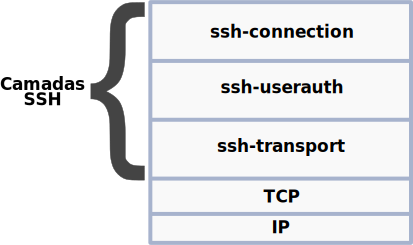
\includegraphics[width=0.3\textwidth]{ssh_layers}
  \caption[Camadas SSH]{Camadas SSH \citep{opensshhood}}
  \label{fig:openssh_layer}
\end{figure}

Dada a enorme importância do OpenSSH, ele é alvo de constantes ataques e,
consequentemente, recebe diversas melhorias do ponto de vista do
desenvolvimentos e de adoção de novas técnicas mais seguras. Como resultado, algumas CVEs
foram criadas e resolvidas no OpenSSH. Dentre as CVEs destacamos:

\begin{description}
  \item [Escalada de privilégios:] Das versões 6.8 até a 6.9 do OpenSSH,
existiu uma vulnerabilidade conhecida como escalada de privilégios
(\emph{privilege escalation}). Este tipo de vulnerabilidade descreve um cenário
na qual um atacante é capaz de enganar o sistema de forma a fazer com que ele
ofereça permissões extras ou de outro usuário. Era possível realizar esse
ataque por meio da opção \texttt{TIOCSTI} passada para a função
\texttt{ioctl()}, que permitia injetar caracteres dentro do terminal do usuário
e assim executar qualquer
comando\footnote{\url{https://cve.mitre.org/cgi-bin/cvename.cgi?name=CVE-2015-6565}}.

  \item [Recuperação de Texto Simples contra cifras CBC:] Quando o OpenSSH utiliza algoritmo de criptografia em bloco em modo
Criptografia de Blocos Encadeados (\emph{Cipher Block Chaining (CBC)}), fica
relativamente simples para um atacante remotamente recuperar pedaços de textos
de blocos criptografados em uma sessão SSH. Essa vulnerabilidade foi mitigada
na versão 5.2 do
OpenSSH\footnote{\url{https://cve.mitre.org/cgi-bin/cvename.cgi?name=CVE-2008-5161}}.

\end{description}

Do ponto de vista do uso de tal aplicação para validar propostas de abstrações
de processos, destacamos que ela pode ser usada para demonstrar ganhos de
segurança e controle de acesso à memória. Uma abordagem é partir de uma versão
antiga do OpenSSH, que não tem a correção para alguma vulnerabilidade, e
demonstrar que a nova abstração sugerida consegue resolver o problema. Note que
os pontos mais fracos do OpenSSH podem ser destacados:

\begin{itemize}
  \item Acesso indevido à chave criptográfica da sessão;
  \item Potencial vazamento de dados;
  \item Escalada de privilégios.
\end{itemize}

\section{Outras Aplicações}

As propostas de novas abstrações de processos podem levar benefícios para
outras áreas além das mostradas nas Seções \ref{sec:web_server} e
\ref{sec:com_enc}. Por esse motivo, apresentamos algumas ferramentas que são de
ampla utilização no mercado e que podem ser utilizadas na validação da
utilidades de algumas das novas abstrações mencionadas no
capítulo~\ref{cap:trabalhos-analisados}.

\subsection{Redis}

Fazer alguns sistemas capazes de operar em grande escala não é uma tarefa trivial e exige constantes
ajustes. Como resultado dessa necessidade, surgiu o sistema Redis, que
implementa a ideia de utilizar um sistema que pode ser um cache e, ao mesmo tempo,
um mecanismo de armazenamento de dados utilizando a memória principal (RAM) com o objetivo
de levar ganhos de desempenho para a aplicação. O Redis também salva os dados
da memória para o disco, o que permite que, posteriormente, ele consiga
reconstruir o sistema na memória.

O Redis é conhecido por utilizar como forma de armazenamento o esquema de
chave-valor (\emph{key-value}). Essa técnica permite o armazenamento dos dados na
forma de um par que consiste de uma chave identificadora e um valor associado a
ela. Quando um valor-chave é salvo, o par passa a estar presente na
RAM. No Redis, uma chave tem que ser uma cadeia de caracteres, mas seus valores podem ser de
vários tipos diferentes. Dentre as abstrações de dados oferecidas por ele, destacam-se:

\begin{itemize}
  \item Lista de strings
  \item Conjunto de strings
  \item Conjunto de strings ordenadas
  \item Tabelas de hash na qual a chave e valor são strings
  \item HyperLogLogs
  \item Stream de entradas com grupos de consumidores
  \item Dados Geoespaciais
\end{itemize}

O tipo utilizado no valor determina qual operação é possível de ser aplicada.
De forma geral, o Redis permite realizar operações de alto nível (p.ex., uniões
e diferenças).

A Figura \ref{fig:redis} apresenta uma visão de geral da organização do Redis.
Repare que ele fornece uma interface de interação do lado do cliente (via
linha de comando ou API) e possui um servidor que é responsável por gerir os dados na memória e em disco.
A implementação faz constante uso da criação de processos (via
chamada de sistema \texttt{fork()}). Basicamente, toda vez que um armazenamento
é necessário, o Redis faz um \texttt{fork()} do processo pai; em seguida, o
processo filho dá início ao processo de escrita em disco enquanto o processo
pai continua realizando as suas tarefas. 

\begin{figure}[!h]
  \centering
  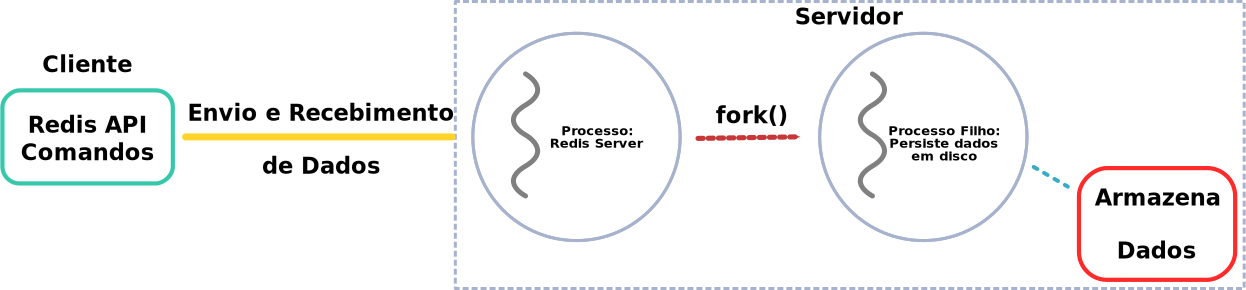
\includegraphics[width=\textwidth]{redis_overview}
  \caption{Visão geral do funcionamento do Redis}
  \label{fig:redis}
\end{figure}

Um dos aspectos mais interessante de Redis, da perspectiva das novas
abstrações de processo é o mecanismo de persistência dos dados. Redis pode
utilizar três: \citep{redisio}: \emph{Relational Database (RDB)},
\emph{Append-Only-File (AOF)} e o comando SAVE. RDB faz uma cópia de todos os
dados presentes na memória para o disco. Por padrão, Redis escreve os dados a
cada dois segundos. Repare que RDB pode causar perda de dados em caso de mau
funcionamento; uma alternativa seria configurá-lo para fazer mais escritas,
contudo isso elevaria consideravelmente o consumo de memória pela natureza do
uso de \texttt{fork()}. AOF registra todas as operações de escrita feitas pelo
servidor, logo tudo é persistido. AOF tem o problema de que pode ser mais lento
do que RDB, a depender da política de sincronização adotada, e também consumir
mais memória.  Por fim, o comando SAVE força o servidor a criar um \emph{dump}
dos dados no momento em que foi solicitado.

% TODO: Vale a pena dar um certo nível de detalhes do código? Não é tão complicado fazer isso, mas preciso ter certeza antes se vale a pena
% Além da referencia do "Redis: under the hood" tem esse artigo aqui: http://robertlehmann.de/img/redis.pdf

Do ponto de vista das novas abstração de processos, o Redis pode ser utilizado
para testar propostas que visam trazer melhorias para a forma como os dados são
compartilhados. Além disso, ele pode ser utilizado para testar formas mais
eficientes e confiável de persistir os dados da memória para o disco.

\subsection{Coleta Automática de Lixo (GC)}
\label{sec:gc}

Várias linguagens de alto nível possuem mecanismos de gerenciamento automático de recursos
(p.ex., memória, processamento paralelo, datas, etc.) que garantem a portabilidade
da aplicação e removem a complexidade de ter que gerenciar recursos de baixo
nível. Dentre as vantagens de tais tecnologias, destacam-se o fato de que o
programador pode manter o foco nas características da aplicação e também a redução
nas chances de erros graves. Java é uma representante desse tipo de
linguagem, fornecendo mecanismos de gerenciamento automático da memória e sendo
portável para múltiplas plataformas. Por uma questão de simplicidade, iremos
adotar Java para as discussões desta seção. Toda a flexibilidade
oferecida por Java deve-se ao uso da \emph{Java Virtual Machine} (JVM), que
fornece elementos para a manipulação dos recursos do SO. Um dos principais
elementos da JVM é o Coletor de Lixo (\emph{Garbage Collector} -- GC), cuja principal tarefa
consiste em abstrair o gerenciamento de memória da aplicação de forma que ela
não tenha que lidar com tal aspecto (alocar e desalocar memória). Dado o seu impacto, o
GC tem sido alvo de constantes otimizações ao longo dos anos e esse é um
elemento que pode se beneficiar de novos recursos oferecidos por extensões às
abstrações de processos.

O coletor de lixo é um módulo que é parte da JVM, executando junto com a aplicação.
Independentemente do algoritmo de gerenciamento de memória implementado pelo
GC, todos eles definem o termo \boldAndIndex{Stop the World (STW)} ou
\emph{Parar tudo} \citep{gc_pauseless}. O STW é uma operação realizada pela
JVM  na qual todas as \emph{threads} da aplicação são suspensas para que o GC execute.
Em outras palavras, a única \emph{thread} executando será a do coletor. Note que o GC
requer essa pausa para funcionar; isso é preciso pois seus algoritmos precisam que
aplicação não faça nenhuma atualização da memória durante uma das fases do
processo de limpeza da memória.

Existem diversos algoritmos que podem ser adotados pelo GC, contudo podemos
generalizar três etapas gerais: \emph{Marking}, \emph{Sweep} e
\emph{Compact}. A etapa de \emph{Marking}, também conhecida por pintura,
consiste em inspecionar os objetos na memória para verificar quais ainda são
considerados ``vivos''. Para determinar se um objeto está vivo, o GC começa por
elementos conhecidos como objetos raiz ou \emph{Garbage Collection Roots}. Os
seguintes componentes são considerados GC roots: variáveis locais,
entrada de parâmetros, \emph{threads} ativas, campos estáticos e referências JNI
\citep{gc_basics}. Partindo de um GC raiz, o GC atravessa o grafo dos objetos
alcançáveis e, para cada elemento que consegue acessar, ele ``pinta'' a referência
como viva. A Figura \ref{fig:gc_alg} ilustra o algoritmo descrito. No contexto
do GC, o processo de parar as \emph{threads} para que a JVM possa executar a etapa de
\emph{Marking} recebe o nome de \emph{safe point} (ponto seguro) e essa
gera um evento STW. O tamanho da pausa é definido pela quantidade de objetos
alcançáveis e seu tamanho no \emph{heap}.

\begin{figure}[!h]
  \centering
  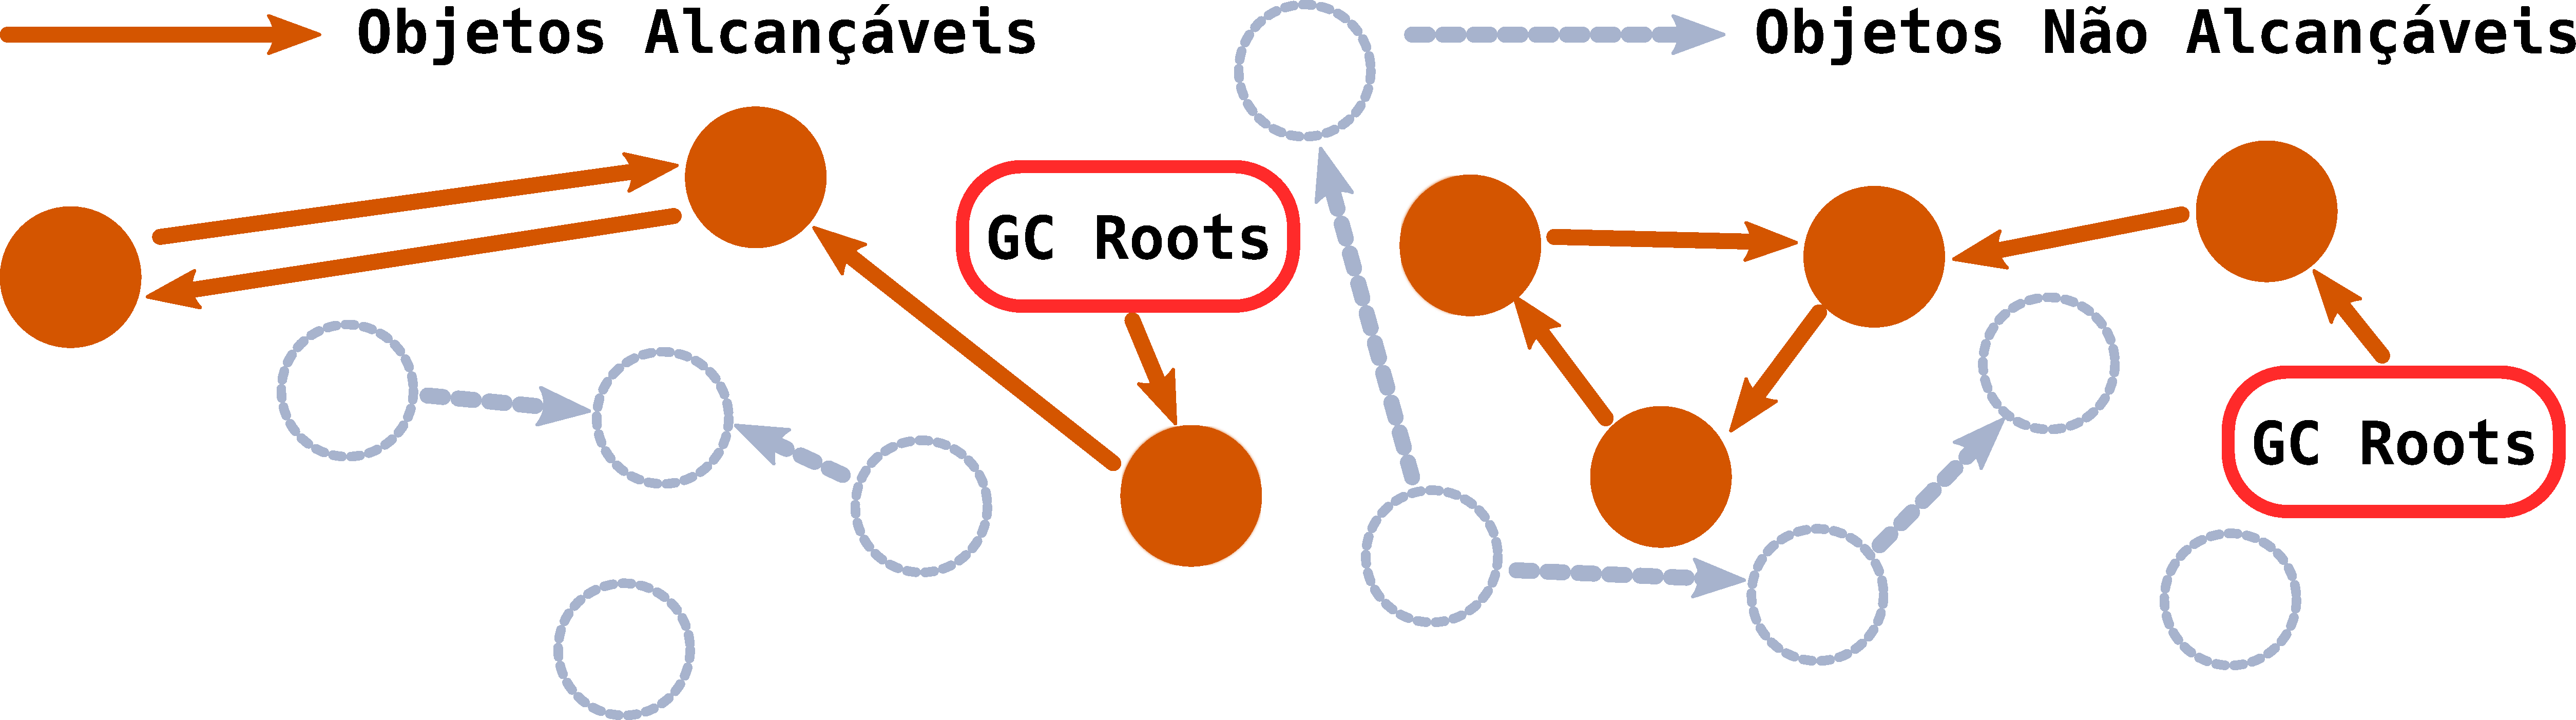
\includegraphics[width=\textwidth]{gc_algoritmo}
	\caption[Algoritmo de pintura da memória]{Algoritmo de pintura da memória\citep{gc_basics}}
  \label{fig:gc_alg}
\end{figure}

Depois da etapa de pintar os objetos na memória, entra em ação a etapa de
remover os objetos que não foram pintados; note que essa etapa pode acontecer
em paralelo ou não, dependendo do algoritmo adotado. O processo de remoção pode
gerar fragmentação na memória, o que pode representar um problema, uma vez que o
GC pode não encontrar espaços de memória grandes o suficiente para outros
objetos. Por isso, também existe uma fase de compactação, na qual o GC realoca os
objetos pintados para liberar espaço contíguo. Contudo, para que a compactação
aconteça corretamente, as referências dos objetos têm que ser atualizadas, uma
vez que a posição física dos objetos mudou. O processo de atualizar as
referências chama-se remapeamento e precisa examinar toda a memória para
realizar os ajustes. Note que a etapa de compactação eleva o tempo de STW. A
Figura \ref{fig:gc_mem} apresenta uma visão da memória durante as três etapas
descritas.

\begin{figure}[!h]
  \centering
  \includegraphics[width=0.8\textwidth]{gc_memory}
	\caption[Visão da memória durante a aplicação do algoritmo de GC]{Visão da memória durante a aplicação do algoritmo de GC\citep{gc_basics}}
  \label{fig:gc_mem}
\end{figure}

Vale salientar que existem diversos algoritmos de GC, cada um com suas
vantagens e desvantagens; nosso objetivo nessa seção é apenas ilustrar o
potencial de uso de tal aplicação para validar novas abstrações de processos.

\section{Discussão Sobre as Aplicações}
\label{sec:disc_app}

Desde o começo deste capítulo até esta seção, apresentamos algumas aplicações
destacando o seu funcionamento, estruturas básicas e os recursos exigidos por
elas. Contudo, o nosso principal objetivo é verificar quais são os tipos de benefícios
e validações que tais aplicações podem fornecer para o avanço das pesquisas em
novas abstrações de processos. Cada tipo de aplicação pode ser útil para
demonstrar algum aspecto da nova abstração, mas idealmente é interessante
evidenciar que as demais aplicações apresentadas também não sofrem com a nova
abstração.

Apache e Nginx são aplicações cujo o objetivo é servir requisições feitas pelos
usuários, ou seja, são servidores web. Esse tipo de aplicação normalmente
oferece opções para que sejam amplamente configuradas de forma a atender os
requisitos do usuário da melhor maneira possível. Tais aplicações são
especializadas para tirar o máximo de proveito possível dos recursos de
hardware, uma vez que servidores web podem lidar com enormes cargas de
requisições levando a um ostensivo uso do hardware. Nesse tipo de aplicação, é
comum que ocorra um amplo consumo da memória e que a CPU esteja próxima do
100\% de utilização em situações de estresse (muitos usuários acessando).  Note
que, quanto mais tempo uma requisição vive, mais memória é consumida, por isso
é desejável que as requisições sejam atendidas o mais rapidamente possível. Por
sua vez, o SO tem que manipular diversos aspectos relacionados à memória,
processos e arquivos. Por esse motivo, utilizar esse tipo de software como
prova de conceito para demonstrar a eficácia de uma nova abstração de processos
é algo extremamente desejável. Essas aplicações podem ser utilizadas para
mostrar que o comportamento da alteração na abstração de processos em uma
situação de alta demanda evidenciando assim o real impacto da nova abstração de
processos. Contudo, é importante ressaltar que os testes realizados em tais
ferramentas devem gerar uma carga substancial (em alguns casos é preciso
alterar as configurações padrão da ferramenta). Esse aspecto é fundamental, uma
vez que não existe grande valor em demonstrar algo usando tais ferramentas com
uma carga pequena, pois isso pouco ajuda na verificação dos reais impactos
gerados pela nova extensão do processo.

Devido ao uso dos módulos de MPM do Apache, é possível testar processos e
\emph{threads} de forma equivalente.  Tal característica é interessante para
comparar novas abstrações diante de dois modos de execução amplamente
utilizados. De forma similar, o Nginx usa outro modelo chamado de \emph{event},
que também representa outro contexto para validação. Da forma como Apache e
Nginx manipulam requisições, podemos dizer que o primeiro fornece um isolamento
horizontal enquanto o segundo proporciona isolamento vertical. O isolamento
horizontal vem do fato de que um processo cria vários outros e o vertical vem
da criação de um único processo por núcleo do processador durante a
inicialização. Ambas as formas de isolamento, horizontal e vertical,  podem ser
úteis para demonstrar que uma nova abstração pode melhorar o isolamento sem
degradar o desempenho.

Apache trabalha com diversos \emph{plugins} que são acoplados ao código
principal dinamicamente. Essa junção tem uma boa relação entre desempenho e
flexibilidade, mas também eleva as chances de quebrar o Apache.  Portanto, o
sistema de \emph{plugins} do Apache fornece um bom elemento de validação para
aquelas abstrações que visam trazer isolamento e recuperação.

Várias propostas de extensão da abstração de processos sugerem algum ganho de
segurança por meio do controle fino ou isolamento de pedaços da memória. Nesse
sentido, OpenSSH e OpenSSL são ferramentas interessantes, já que possuem os
requisitos de segurança adequados para a validação das novas abstrações. Em
especial, ambas as aplicações tem diversas CVEs associadas a si com correções
disponíveis a partir de uma versão específica. Portanto, uma proposta de
melhoria na abração de processo que eleva a segurança pode demonstrar o seu
real valor em uma dessas aplicações.

Redis, por sua vez, é uma aplicação que trabalha com grandes quantidade de
dados na memória e que tem excelente desempenho em situações de forte
demanda. Essas características fazem dele uma excelente ferramenta para
demonstrar novas técnicas de compartilhamento da memória. Além disso, um dos
objetivos de Redis é auxiliar na escalabilidade das aplicações. Por isso, é
desejável que ele reaja rapidamente a qualquer problema. Nesse contexto,
abstrações de processos novas que tragam melhorias no tempo recuperação de uma
aplicação em caso de falha podem usar o Redis com instrumento de validações.

Novas abstrações de processos podem entregar ganhos de desempenho para as
aplicações por utilizar algum recurso de hardware ou mesmo fornecer uma nova
estrutura de dados para a aplicação. Tal otimização pode ser demonstrada em um
GC, uma vez que esse tipo de aplicação faz uso de vários algoritmos que dependem
de certos dados fornecidos pelo SO. Como exemplo disto, a fase de compactação
pode ser otimizada se o endereço virtual for mantido e apenas o endereço físico
alterado \citep{pauseless}.

A Tabela \ref{tab:app_alvos} busca resumir quais aplicações podem ser usadas
para demonstrar algum aspecto da nova abstração de processos. Além disso, esta
seção inteira responde a pergunta RQ3, uma vez que apresenta e discute diversas
aplicações. Por fim, repare na Tabela \ref{tab:app_alvos} que Apache é uma das
ferramentas que melhor pode ser usada para demonstrar os aspectos de uma nova
abstração de processos. No Capítulo \ref{cap:estudo-de-caso} aprofundamos a
validação utilizando Apache para testar o MVAS.

\begin{table}[]
\small
\centering
  \begin{tabular}{|@{}c@{}|@{}c@{}|@{}c@{}|@{}c@{}|@{}c@{}|@{}c@{}|@{}c@{}|}
  % TOPO DA TABELA
  % |M{2.5cm}|M{2.5cm}|M{2.5cm}|
  \hline
  \multicolumn{1}{|l|}{\diagbox[width=2.5cm, height=2cm]{App}{Alvo}} &
    % Troca de contexto
    \multicolumn{1}{@{}c@{}|}{\begin{tabular}[c]{@{}c@{}}Controle\\fino da\\Memória\end{tabular}} &
    % Persistência de processos
    \multicolumn{1}{@{}c@{}|}{\begin{tabular}[c]{@{}c@{}}Consumo\\ de CPU \end{tabular}} &
    % Controle fino de privilégios
    \multicolumn{1}{@{}c|}{\begin{tabular}[c]{@{}c@{}}Consumo \\de Memória \end{tabular}} &
    % Segurança
    \multicolumn{1}{@{}c|}{Segurança} &
    % Recuperação
    \multicolumn{1}{@{}c|}{Recuperação} &
    % Otimização
    \multicolumn{1}{@{}c|}{Otimização} \\ \hline \hline
  % Início da tabela
  Apache  &                             & \ding{52}\ding{52}\ding{52} & \ding{52}\ding{52}\ding{52} & \ding{52}\ding{52}            & \ding{52}\ding{52} & \ding{52}\ding{52}          \\ \hline
  Nginx   & \ding{52}                   & \ding{52}\ding{52}          & \ding{52}\ding{52}          & \ding{52}                     & \ding{52}          & \ding{52}\ding{52}          \\ \hline
  OpenSSL & \ding{52}\ding{52}\ding{52} &                             &                             & \ding{52}\ding{52}\ding{52}   &                    &                             \\ \hline
  OpenSSH & \ding{52}\ding{52}\ding{52} &                             &                             & \ding{52}\ding{52}\ding{52}   &                    &                             \\ \hline
  Redis   &  \ding{52}\ding{52}         &                             & \ding{52}\ding{52}          &                               & \ding{52}          & \ding{52}                   \\ \hline
  GC      &                             & \ding{52}                   & \ding{52}\ding{52}          &                               &                    & \ding{52}\ding{52}\ding{52} \\ \hline
  \end{tabular}
\caption{Relação aplicações e alvos}
\label{tab:app_alvos}
\end{table}


\section{Microbenchmarks}
\label{sec:micro}

\emph{Microbenchmarks} têm por objetivo mensurar e fornecer meios para
analisar uma única característica do objeto de estudo. Eles
facilitam o processo de desenvolvimento,
mostram o impacto em um único elemento de forma a facilitar a análise e são
relativamente simples de serem implementados. Contudo, a principal desvantagem
encontra-se no fato de que eles não ajudam a revelar o impacto geral do objeto
alvo. Por esse motivo, é interessante trabalhar com um conjunto de
\emph{microbenchmarks} e também com validações usando aplicações (como
descrito na Seção \ref{sec:disc_app}). Expandindo o contexto dos
\emph{microbenchmarks} para o subconjunto da pesquisa sobre abstrações de
processos, queremos destacar aquelas validações que lidam com a memória,
sobrecargas extra e impactos na utilização de certos recursos de hardware.

No Capítulo \ref{cap:trabalhos-analisados}, apresentamos diversas propostas que
buscam de alguma maneira lidar com os mecanismos de acesso à memória. Várias
dessas propostas permitem o controle fino da memória ou algum ganho de
segurança que os autores normalmente demonstram por meio da alteração de
algumas aplicações (p.ex., OpenSSL ou OpenSSH). Contudo, alterações no
gerenciamento da memória podem incorrer em erros e em problemas de desempenho.
Nesse sentido, alguns \emph{microbenchmarks} podem ser extremamente oportunos
para validar o uso de novas abstrações de processos que lidam com a memória.
Com base em todos os trabalhos analisados no Capítulo
\ref{cap:trabalhos-analisados}, extraímos os seguintes itens:

\begin{description}

  \item[Medir tempo gasto com novos mecanismos de alocação de memória:]

Algumas propostas criam mecanismos de alocação de memória contendo
características novas, por isso é interessante comparar os mecanismos
propostos pelo pesquisador utilizando como base a forma padrão de alocação
(p.ex., \texttt{malloc()} e \texttt{calloc()}). Tendo os valores base extraídos
das operações já consolidadas e os valores coletados do modelo proposto,
torna-se possível ter um critério para compreender o real impacto da mudança.
Vale observar que esse tipo de \emph{microbenchmark} precisa ser feito com
múltiplas cargas de tamanhos variados; no mínimo, espera-se cargas na ordem dos
KBs, MBs e GBs.

  \item[Medir tempo gasto com operações de litura e escrita:]

Mensurar o tempo de leitura e escrita em memória usando os mecanismos
padrão é importante para obter o custo de acesso base. Tal informação deve ser
utilizada para comparar com novas propostas de abstrações de processos que
adicionam camadas extras para acessar a memória (p.ex., Nooks e Wedge).
Novamente, é importante que várias cargas de trabalho sejam utilizadas.

\end{description}

Algumas propostas sugerem a adição de novas chamadas de sistema que adicionam
novos modelos de programação (p.ex., lwC e MVAS). Apesar de as chamadas de sistema
serem relativamente rápidas, elas adicionam \emph{overhead}. Por isso, é
desejável que o pesquisador identifique alguma \emph{syscall} padrão que tenha
algum nível de similaridade com a nova chamada que ele está propondo; assim, ele
pode realizar medições do tempo total gasto com a chamada padrão para ter um valor
base para comparar com a nova chamada. Contudo, existem casos em que a nova
chamada representa algo totalmente novo e em que não faz sentido comparar com
qualquer outra chamada já existente. Independentemente de existir ou não uma
chamada base, é desejável que o pesquisador execute \emph{microbenchmarks} que
possam aferir:

\begin{description}
  \item [Tempo total gasto na chamada:]

Espera-se que o tempo total da chamada seja medido, considerando-se cenários em
que a chamada é feita dezenas, centenas e milhares de vezes. Esse tipo de
parametrização é importante na validação do comportamento da chamada sob
diferentes cargas.

  \item [Tempo total gasto na chamada em um contexto de concorrência:]

Testes realizados no contexto de concorrência auxiliam na validação de como
novas chamadas se comportam. Novamente, espera-se que tal teste execute
a nova chamada diversas vezes.

  \item [Quantidade de trocas de contexto:]

As novas instruções podem fazer com que o número de trocas de contexto aumente,
por isso é valioso medir tal aspecto referente à nova chamada.

\end{description}

Várias propostas propõem um novo hardware (p.ex., Mondrix) ou uma mudança na
forma como um dispositivo é usado, o que torna importante validar alguns
aspectos de uso. Contudo, para a questão do \emph{microbenchmark} vamos
considerar apenas os aspectos referentes à reutilização do hardware de
virtualização, uma vez que consideramos que tal técnica tem amplas chances de
ser adotada (discutimos esse aspecto com mais detalhes no Capítulo
\ref{cap:analise-sobre-abstracoes-de-processos}). Nesse contexto, dois
elementos devem ser medidos:

\begin{description}

  \item [Custos de operações que executam \emph{VM Entry} e \emph{Exit}:]

Chamadas que utilizam recursos de virtualização têm custos para entrar e sair
do kernel. Mensurar tal custo é útil para analisar em quais contextos vale a pena
ou não utilizar os recursos de virtualização.

  \item [Medir o uso de EPT:]

Quando se utiliza a EPT, espera-se que o total de \emph{TLB misses} se eleve,
uma vez que, em muitos casos, é preciso procurar por dois níveis de chamadas
~\citep{belay}. Portanto, torna-se interessante medir o tempo total gasto
quando a EPT é usada sob diferentes cargas.

\end{description}

Por fim, é importante ressaltar que vários dos \emph{microbenchmarks} devem
utilizar recursos estatísticos para derivar seus resultados. Por exemplo,
espera-se que cada experimento execute múltiplas vezes e a sua média ou mediana
e intervalo de confiança sejam calculados. Além disso, a combinação de
múltiplos \emph{microbenchmarks} pode auxiliar consideravelmente na validação
de uma nova proposta de abstração.

\section{Discussão}

Recapitulando o objetivo deste Capítulo por meio das perguntas de pesquisa:

\begin{quote}
  \item \emph{QP3:.} ``Quais aplicações podem ser utilizadas para avaliar as novas abstrações adicionadas a um SO?''
  \item \emph{QP4:.} ``Qual conjunto de \emph{microbenchmarks} pode ser utilizado para auxiliar a entender os impactos de uma nova característica adicionada às abstrações de processos?''
\end{quote}

Para responder a primeira pergunta, fizemos uma jornada da Seção
\ref{sec:web_server} até a \ref{sec:disc_app} analisando diversas aplicações
amplamente consolidadas. Em especial, a Seção \ref{sec:disc_app} apresentou uma
discussão sobre as vantagens em se utilizar as aplicações para validar as novas
abstrações de processos. A Tabela \ref{tab:app_alvos} buscou relacionar as
aplicações e as áreas que elas auxiliam a validar.

Para responder a segunda pergunta, revisitamos todos os trabalhos e buscamos
compilar um conjunto de \emph{microbenchmarks} que auxiliam no processo de
validação.  A combinação de múltiplos \emph{microbenchmarks} auxilia
mostrando o impacto da alteração de forma mais abrangente, contudo, esse tipo
de validação sozinho não é capaz de revelar os impactos gerais de uma nova
abstração.

Em um cenário ideal, a combinação das validações utilizando as aplicações
discutidas em conjunto com os \emph{microbenchmarks} representa uma boa
cobertura sobre os impactos de uma nova abstração. Por fim, é importante
relembrar que tais validações devem buscar utilizar cargas de trabalho
relevantes para tornar claros os impactos da nova abstração.
